\documentclass[letterpaper]{article}
\usepackage[margin=1in]{geometry}
\usepackage[utf8]{inputenc}
\usepackage{textcomp}
\usepackage{amssymb}
\usepackage{natbib}
\usepackage{graphicx}
\usepackage{gensymb}
\usepackage{amsthm, amsmath, mathtools}
\usepackage[dvipsnames]{xcolor}
\usepackage{enumerate}
\usepackage{mdframed}
\usepackage[most]{tcolorbox}
\usepackage{csquotes}
% https://tex.stackexchange.com/questions/13506/how-to-continue-the-framed-text-box-on-multiple-pages

\tcbuselibrary{theorems}

\newcommand{\R}{\mathbb{R}}
\newcommand{\Z}{\mathbb{Z}}
\newcommand{\N}{\mathbb{N}}
\newcommand{\Q}{\mathbb{Q}}
\newcommand{\C}{\mathbb{C}}
\newcommand{\code}[1]{\texttt{#1}}
\newcommand{\mdiamond}{$\diamondsuit$}
\newcommand{\PowerSet}{\mathcal{P}}
\newcommand{\Mod}[1]{\ (\mathrm{mod}\ #1)}
\DeclareMathOperator{\lcm}{lcm}

%\newtheorem*{theorem}{Theorem}
%\newtheorem*{definition}{Definition}
%\newtheorem*{corollary}{Corollary}
%\newtheorem*{lemma}{Lemma}
\newtheorem*{proposition}{Proposition}


\newtcbtheorem[number within=section]{theorem}{Theorem}
{colback=green!5,colframe=green!35!black,fonttitle=\bfseries}{th}

\newtcbtheorem[number within=section]{definition}{Definition}
{colback=blue!5,colframe=blue!35!black,fonttitle=\bfseries}{def}

\newtcbtheorem[number within=section]{corollary}{Corollary}
{colback=yellow!5,colframe=yellow!35!black,fonttitle=\bfseries}{cor}

\newtcbtheorem[number within=section]{lemma}{Lemma}
{colback=red!5,colframe=red!35!black,fonttitle=\bfseries}{lem}

\newtcbtheorem[number within=section]{example}{Example}
{colback=white!5,colframe=white!35!black,fonttitle=\bfseries}{def}

\newtcbtheorem[number within=section]{note}{Important Note}{
        enhanced,
        sharp corners,
        attach boxed title to top left={
            xshift=-1mm,
            yshift=-5mm,
            yshifttext=-1mm
        },
        top=1.5em,
        colback=white,
        colframe=black,
        fonttitle=\bfseries,
        boxed title style={
            sharp corners,
            size=small,
            colback=red!75!black,
            colframe=red!75!black,
        } 
    }{impnote}
\usepackage[utf8]{inputenc}
\usepackage[english]{babel}
\usepackage{fancyhdr}
\usepackage[hidelinks]{hyperref}

\pagestyle{fancy}
\fancyhf{}
\rhead{Math 170A}
\chead{March 13th, 2023}
\lhead{Course Notes}
\rfoot{\thepage}

\setlength{\parindent}{0pt}

\newcommand{\0}{\mathbf{0}}
\newcommand{\y}{\mathbf{y}}
\renewcommand{\b}{\mathbf{b}}
\newcommand{\x}{\mathbf{x}}
\newcommand{\e}{\mathbf{e}}
\newcommand{\rr}{\mathbf{r}}
\newcommand{\vv}{\mathbf{v}}
\renewcommand{\u}{\mathbf{u}}

\begin{document}

\begin{titlepage}
    \begin{center}
        \vspace*{1cm}
            
        \Huge
        \textbf{Math 170A Notes}
            
        \vspace{0.5cm}
        \LARGE
        Introduction to Numerical Analysis: Linear Algebra
            
        \vspace{1.5cm}
            
        \vfill
            
        Winter 2023\\
        Taught by Professor Shuang Liu
    \end{center}
\end{titlepage}

\pagenumbering{gobble}

\newpage 

\pagenumbering{gobble}
\begingroup
    \renewcommand\contentsname{Table of Contents}
    \tableofcontents
\endgroup

\newpage
\pagenumbering{arabic}

\section{Matrix Multiplication (Section 1.1)}
Consider an $n \times m$ matrix, or a matrix with $n$ rows and $m$ columns:
\[
    A = \begin{bmatrix}
        a_{11} & a_{12} & \hdots & a_{1m} \\ 
        a_{21} & a_{22} & \hdots & a_{2m} \\ 
        \vdots & \vdots &        & \vdots \\ 
        a_{n1} & a_{n2} & \hdots & a_{nm}
    \end{bmatrix}.
\]
The entries of $A$ might be real or complex numbers although, for now, we'll assume they're real. Suppose we have an $m$-tuple (or vector) of real numbers: 
\[\mathbf{x} = \begin{bmatrix}
    x_1 \\ x_2 \\ \vdots \\ x_m
\end{bmatrix}.\]

\subsection{Multiplying Matrix by Vector}
Suppose $A$ is an $n \times \boxed{m}$ matrix and $\mathbf{x}$ is a vector with $m$ elements (i.e., a $\boxed{m} \times 1$ matrix). Let's suppose we wanted to find $A\mathbf{x}$. There are two ways we can do this. 

\subsubsection{Solving as a Single Component}
We can solve for
\[A\mathbf{x} = \mathbf{b},\]
where 
\[\mathbf{b} = \begin{bmatrix}
    b_1 \\ b_2 \\ \vdots \\ b_n
\end{bmatrix}.\]
Here, 
\[b_i = a_{i1} x_1 + a_{i2} x_2 + \hdots + a_{im} x_{m} = \sum_{j = 1}^{m} a_{ij} x_j.\]

\begin{mdframed}
    (Example.) Consider
    \[A = \begin{bmatrix}
        1 & 2 & 3 \\ 
        4 & 5 & 6
    \end{bmatrix} \qquad \mathbf{x} = \begin{bmatrix}
        7 \\ 8 \\ 9
    \end{bmatrix}.\]
    We note that 
    \[A\mathbf{x} = \begin{bmatrix}
        b_1 \\ 
        b_2
    \end{bmatrix},\]
    where 
    \[b_1 = a_{11}x_1 + a_{12}x_2 + a_{13}x_3 = 1(7) + 2(8) + 3(9) = 50\]
    and 
    \[b_2 = a_{21}x_1 + a_{22}x_2 + a_{23}x_3 = 4(7) + 5(8) + 6(9) = 122.\]
\end{mdframed}
We can write some code to perform this operation for us:
\begin{algorithmic}
    \State $\mathbf{b} \gets \mathbf{0}$
    \For{$i = 1, \hdots, n$}
        \For{$i = 1, \hdots, m$}
            \State $b_i \gets b_i + a_{ij} x_j$
        \EndFor
    \EndFor
\end{algorithmic}
Note that the $j$-loop accumulates the inner product $b_i$. 
    
\subsubsection{Solving as a Formula}
We can also solve for $A\mathbf{x} = \mathbf{b}$ by considering the following:
\[\begin{bmatrix}
    b_1 \\ b_2 \\ \vdots \\ b_n 
\end{bmatrix} = \begin{bmatrix}
    a_{11} \\ a_{21} \\ \vdots \\ a_{n1}
\end{bmatrix} x_1 + \begin{bmatrix}
    a_{12} \\ a_{22} \\ \vdots \\ a_{n2}
\end{bmatrix} x_2 + \hdots + \begin{bmatrix}
    a_{1m} \\ a_{2m} \\ \vdots \\ a_{nm}
\end{bmatrix} x_m.\]
This shows that $\mathbf{b}$ is a linear combination of the columns of $A$. 

\begin{mdframed}
    (Example.) Consider
    \[A = \begin{bmatrix}
        1 & 2 & 3 \\ 
        4 & 5 & 6
    \end{bmatrix} \qquad \mathbf{x} = \begin{bmatrix}
        7 \\ 8 \\ 9
    \end{bmatrix}.\]
    Using this approach, we now have 
    \[\begin{bmatrix}
        1 \\ 4
    \end{bmatrix} 7 + \begin{bmatrix}
        2 \\ 5
    \end{bmatrix} 8 + \begin{bmatrix}
        3 \\ 6
    \end{bmatrix} 9 = \begin{bmatrix}
        7 \\ 28
    \end{bmatrix} + \begin{bmatrix}
        16 \\ 40
    \end{bmatrix} + \begin{bmatrix}
        27 \\ 54
    \end{bmatrix} = \begin{bmatrix}
        50 \\ 122
    \end{bmatrix}.\]
\end{mdframed}

\begin{proposition}
    If $\mathbf{b} = A\mathbf{x}$, then $\mathbf{b}$ is a linear combination of the columns of $A$. If we let $A_j$ denote the $j$th column of $A$, we have 
    \[\mathbf{b} = \sum_{j = 1}^{m} A_j x_j.\]
\end{proposition}
We can also express this as pseudocode: 
\begin{algorithmic}
    \State $\mathbf{b} \gets \mathbf{0}$
    \For{$j = 1, \hdots, m$}
        \State $\mathbf{b} \gets \mathbf{b} + A_j x_j$
    \EndFor
\end{algorithmic}
If we use a loop to perform each vector operation, the code becomes:
\begin{algorithmic}
    \State $\mathbf{b} \gets \mathbf{0}$
    \For{$j = 1, \hdots, m$}
        \For{$i = 1, \hdots, n$}
            \State $b_i \gets b_i + a_{ij} x_j$
        \EndFor 
    \EndFor
\end{algorithmic}
Notice how the loops for rows and columns are interchangeable.

\subsection{Flop Counts}
We note that real numbers are normally stored in computers in a floating-point format. The arithmetic operations that a computer performs on these numbers are called \emph{floating-point operations}, or \emph{flops}. So, 
\[b_i \gets b_i + a_{ij}x_j\]
involves two flops: one floating-point multiply and one floating-point add. \textbf{Essentially}, we would like to count the number of operations on real numbers, or the number of addition, subtraction, multiplication, and division operations, within our program.

\begin{mdframed}
    (Example.) Consider 
    \[\mathbf{v} = \begin{bmatrix}
        v_1 \\ v_2 \\ \vdots \\ v_n
    \end{bmatrix} \qquad \mathbf{w} = \begin{bmatrix}
        w_1 \\ w_2 \\ \vdots \\ w_n
    \end{bmatrix}.\]
    Let's compute the inner product\footnote{A generalization of the dot product}:
    \begin{equation*}
        \begin{aligned}
            \cyclic{\mathbf{v}, \mathbf{w}} &= \mathbf{v}^T \cdot \mathbf{w} = \begin{bmatrix}
                v_1 & v_2 & \hdots & v_n
            \end{bmatrix} \begin{bmatrix}
                w_1 \\ w_2 \\ \vdots \\ w_n
            \end{bmatrix} \\ 
                &= v_1 \cdot w_1 + v_2 \cdot w_2 + \hdots + v_n \cdot w_n \\ 
                &= \sum_{i = 1}^{n} v_i w_i.
        \end{aligned}
    \end{equation*}
    There are $n - 1$ addition operations and $n$ multiplication operations, for a total of $2n - 1$ flop count.
\end{mdframed}

\subsubsection{Big-O Notation}
We note that $\mathbf{v}^T \mathbf{w}$, where $\mathbf{v}, \mathbf{w} \in \R^n$ needs $2n$ flops. This is the same thing as saying that the operation takes $\BigO(n)$ time as $n \mapsto \infty$. This means that we can disregard the implied constant, which is 2 in this case. The reason why we can do this is because, as $n$ grows larger, the constant doesn't really matter all that much. 

\bigskip 

For instance, if $n$ is large, then $\BigO(n)$ is faster than $\BigO(n^2)$, and $\BigO(n^2)$ is faster than $\BigO(n^3)$. 


\section{Systems of Linear Equations (Section 1.2)}
This section is mainly going to be reviewing systems of linear equations.

\subsection{Nonsingularity and Uniqueness of Solutions}
Suppose we have a system of $n$ linear equations and $n$ unknowns
\begin{equation} \label{1-14:1}
    \begin{split}
        a_{11}x_1 + a_{12}x_2 + &\hdots + a_{1n}x_n = b_1 \\
        a_{21}x_1 + a_{22}x_2 + &\hdots + a_{2n}x_n = b_2 \\
        &\vdots \\
        a_{n1}x_1 + a_{n2}x_2 + &\hdots + a_{nn}x_n = b_n.
    \end{split}
\end{equation}
We're given the coefficients $a_{ij}$ and $b_i$, and we want to find $x_1, \hdots, x_n$ that satisfies the equations. Generally, it's tedious to write (\ref{1-14:1}) over and over again, so we might write it as a single matrix equation 
\begin{equation} \label{1-14:2}
    A\x = \b,
\end{equation}
where 
\[A = \begin{bmatrix}
    a_{11} & a_{12} & \hdots & a_{1n} \\ 
    a_{21} & a_{22} & \hdots & a_{2n} \\ 
    \vdots & \vdots &        & \vdots \\ 
    a_{n1} & a_{n2} & \hdots & a_{nn}
\end{bmatrix} \quad \x = \begin{bmatrix}
    x_1 \\ x_2 \\ \vdots \\ x_n
\end{bmatrix} \quad \b = \begin{bmatrix}
    b_1 \\ b_2 \\ \vdots \\ b_n
\end{bmatrix}.\]
In other words, we are given $A$ and $\b$ and must solve for $\x$. $A \in \R^{n \times n}$ is an $n \times n$ matrix, also known as a \emph{square matrix}.

\bigskip 

Note that (\ref{1-14:2}) has a unique solution if and only if the matrix $A$ is nonsingular. 

\begin{theorem}{}{1-14:3}
    Let $A$ be a square matrix. The following six conditions are equivalent; that is, if any one holds, they all hold: 
    \begin{enumerate}[(a)]
        \item $A^{-1}$ exists. 
        \item There is no nonzero $\mathbf{y}$ such that $A\mathbf{y} = \mathbf{0}$.
        \item The columns of $A$ are linearly independent.
        \item The rows of $A$ are linearly independent. 
        \item $\det(A) \neq 0$.
        \item Given any vector $b$, there is exactly one vector $\x$ such that $A\x = \b$. 
    \end{enumerate}
\end{theorem}
\textbf{Remark:} Existence and uniqueness of $\x$ only depends on $A$ and not on $\b$.

To briefly review the inverse of a matrix, we should note that the $n \times n$ \textbf{identity matrix} is denoted by $I$, and is the unique matrix such that 
\[AI = IA = A\]
for all $A \in \R^{n \times x}$.The identity matrix has \code{1}'s on its main diagonal and \code{0}'s everywhere else. For example, the $3 \times 3$ identity matrix has the form 
\[I = \begin{bmatrix}
    1 & 0 & 0 \\ 
    0 & 1 & 0 \\ 
    0 & 0 & 1
\end{bmatrix}.\]
Given a matrix $A$, if there is a matrix $B$ such that $AB = BA = I$, the $B$ is called the inverse of $A$ and is denoted $A^{-1}$. \emph{Not every matrix will have an inverse.}

\bigskip 

In any case, if the conditions of Theorem \ref{th:1-14:3} hold, $A$ is said to be nonsingular or invertible. If the conditions do \emph{not} hold, then $A$ is said to be singular or noninvertible. In this case, (\ref{1-14:2}) will have no solution or infinitely many solutions. 

\bigskip 

Now, we'll focus on when $A$ is nonsingular. In this case, the unique solution of \ref{1-14:2} can be obtained by multiplying both sides by $A^{-1}$. We can see this from how 
\begin{equation*}
    \begin{aligned}
        A\x &= \b \\ 
            &\implies A^{-1} A \x = A^{-1} \b \\ 
            &\implies I\x = A^{-1}\b \\ 
            &\implies \x = A^{-1}\b. 
    \end{aligned}
\end{equation*}
While this is guaranteed to solve the problem, doing so is a bad idea as it's very error-prone. It's usually a better idea to solve $A\x = \b$. It should also be noted that computing $A^{-1}$ is computationally expensive.

\bigskip 

\textbf{Note:} We can use MATLAB to solve for $\x$ by using 
\begin{verbatim}
    x = A \ b\end{verbatim}

\subsection{Numerical (Approximate) Solution of Differential Equations}
In this section, we'll focus on ordinary differential equations (ODE). These contain one or more functions of one independent variable and the derivatives of those functions. For example, consider the initial value system 
\begin{equation}\label{1-14:4}
    \begin{cases}
        u'(x) + au(x) = f(x) \\ 
        u(0) = 0
    \end{cases}
\end{equation}
with $x \in [0, 1]$. We have two functions, $f(x)$ and $u(x)$, derivative $u'(x)$, and one independent variable $x$. Suppose a fixed $a \in \R$ and $f: \R \mapsto \R$. Our goal is to find a function $u$ satisfying the system (\ref{1-14:4}).

\begin{enumerate}
    \item First, approximate $u'$. 
    \[u'(x) = \lim_{h \mapsto 0} \frac{u(x + h) - u(x)}{h} = \lim_{h \mapsto 0} \frac{u(x) - u(x - h)}{h} = \lim_{h \mapsto 0} \frac{u(x + h) - u(x - h)}{2h}.\]
    We want to pick a very small $h$ to do this evaluation. That way, for a small enough $h$ (close to 0), we can do 
    \begin{equation}\label{1-14:5}
        u'(x) \approx \frac{u(x + h) - u(x)}{h} \approx \frac{u(x) - u(x - h)}{h} \approx \frac{u(x + h) - u(x - h)}{2h}
    \end{equation}

    \item To choose a small $h$, we can divide the given interval, which in this case is $[0, 1]$, into $m$ subintervals. Pick a (possibly large) $m \in \N$, and then subdivide the interval into $m$ equal subintervals of length $h = \frac{1}{m}$. 
    
    \begin{center}
        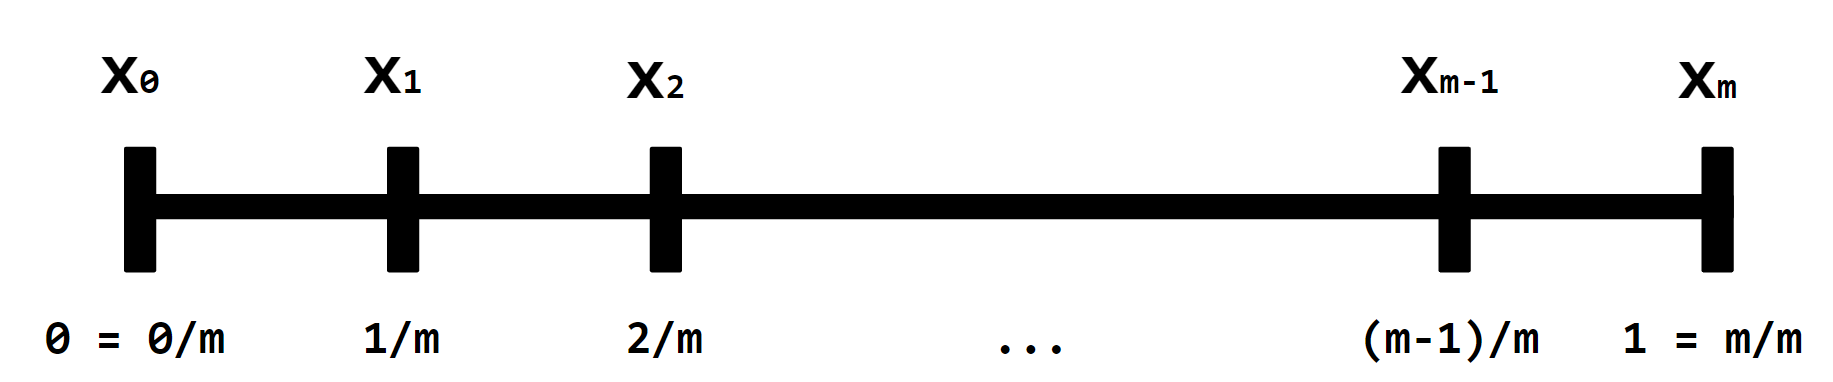
\includegraphics[scale=0.4]{assets/sub_divide.png}
    \end{center}
    
    The subdivision points of the intervals would be $x_i = \frac{i}{m}$ for $i = 0, 1, 2, \hdots, m$. That way, we can find $u$ on those points; that is, we can find \[u\left(x_i = \frac{i}{m}\right).\] 
    With this in mind, the approximation formula from (\ref{1-14:5}) can be rewritten as such:
    \[u'(x_i) \approx \frac{u(x_i + h) - u(x_i)}{h} \approx \frac{u(x_i) - u(x_i - h)}{h} \approx \frac{u(x_i + h) - u(x_i - h)}{2h},\]
    or just 
    \[u'(x_i) \approx \frac{u(x_{i + 1}) - u(x_{i})}{h} \approx \frac{u(x_i) - u(x_{i - 1})}{h} \approx \frac{u(x_{i + 1}) - u(x_{i - 1})}{2h}.\] 
    The approximation used depends on the information you are given.
    \item Now, we can set up a linear system. We want to find $u(x_i)$ for all $i \in [0, m]$. 
    \begin{itemize}
        \item For $i = 0$, it's clear that 
        \[u(x_i) = u(x_0) = u(0) = 0\]
        from the given condition.

        \item For $i = 1$, we can use the approximation 
        \[u'(x_i) \approx \frac{u(x_i) - u(x_{i - 1})}{h}\]
        to get 
        \begin{equation*}
            \begin{aligned}
                &\frac{u(x_1) - u(x_0)}{h} + au(x_1) = f(x_1) \\ 
                    &\implies \frac{u(x_1) - u(0)}{\frac{1}{m}} + au(x_1) = f(x_1) \\ 
                    &\implies mu(x_1) + au(x_1) = f(x_1) \\ 
                    &\implies mu\left(\frac{1}{m}\right) + au\left(\frac{1}{m}\right) = f\left(\frac{1}{m}\right) \\ 
                    &\implies u\left(\frac{1}{m}\right) (m + a) = f\left(\frac{1}{m}\right) \\ 
                    &\implies u\left(\frac{1}{m}\right) = \frac{f\left(\frac{1}{m}\right)}{m + a}
            \end{aligned}
        \end{equation*}

        \item For $i = 2$, we can use the approximation
        \[u'(x_i) \approx \frac{u(x_i) - u(x_{i - 1})}{h}\]
        to get 
        \begin{equation*}
            \begin{aligned}
                &\frac{u(x_2) - u(x_1)}{h} + au(x_2) = f(x_2) \\ 
                    &\implies \frac{u(x_2) - u(x_1)}{\frac{1}{m}} + au(x_2) = f(x_2) \\ 
                    &\implies m\left(u(x_2) - u(x_1)\right) + au(x_2) = f(x_2) \\ 
                    &\implies mu(x_2) - mu(x_1) + au(x_2) = f(x_2) \\ 
                    &\implies u(x_2)(m + a) - mu(x_1) = f(x_2) \\ 
                    &\implies u(x_2)(m + a) = mu(x_1) + f(x_2) \\ 
                    &\implies u(x_2) = \frac{mu(x_1) + f(x_2)}{m + a} \\ 
                    &\implies u\left(\frac{2}{m}\right) = \frac{mu\left(\frac{1}{m}\right) + f\left(\frac{2}{m}\right)}{m + a}.
            \end{aligned}
        \end{equation*}
        Note that we found $u\left(\frac{1}{m}\right)$ in the previous step.

        \item For $i = m$, we have 
        \begin{equation*}
            \begin{aligned}
                &\frac{u(x_m) - u(x_{m - 1})}{h} + au(x_m) = f(x_m) \\ 
                    &\implies \frac{u(1) - u(x_{m - 1})}{\frac{1}{m}} + au(1) = f(1) \\ 
                    &\implies m(u(1) - u(x_{m - 1})) + au(1) = f(1) \\ 
                    &\implies mu(1) - mu(x_{m - 1}) + au(1) = f(1) \\ 
                    &\implies u(1)(m + a) - mu(x_{m - 1}) = f(1) \\ 
                    &\implies u(1)(m + a) = mu(x_{m - 1}) + f(1) \\ 
                    &\implies u(1) = \frac{mu(x_{m - 1}) + f(1)}{m + a} \\ 
                    &\implies u(1) = \frac{mu(\frac{m - 1}{m}) + f(1)}{m + a}.
            \end{aligned}
        \end{equation*}
    \end{itemize}
\end{enumerate}

With this all in mind, we want to be able to generate a linear system of the form 
\begin{equation*}
    \begin{aligned}
        &\begin{cases}
            u\left(\frac{1}{m}\right) = \frac{f\left(\frac{1}{m}\right)}{m + a} \\ 
            u\left(\frac{2}{m}\right) = \frac{mu\left(\frac{1}{m}\right) + f\left(\frac{2}{m}\right)}{m + a} \\ 
            \vdots \\ 
            u(1) = \frac{mu(\frac{m - 1}{m}) + f(1)}{m + a}
        \end{cases} \\ 
        &\implies \begin{cases}
            (m + a) u\left(\frac{1}{m}\right) = f\left(\frac{1}{m}\right) \\ 
            (m + a) u\left(\frac{2}{m}\right) = mu\left(\frac{1}{m}\right) + f\left(\frac{2}{m}\right) \\ 
            \vdots \\ 
            (m + a) u(1) = mu(\frac{m - 1}{m}) + f(1)
        \end{cases} \\ 
        &\implies \begin{cases}
            (m + a) u\left(\frac{1}{m}\right) = f\left(\frac{1}{m}\right) \\ 
            -mu\left(\frac{1}{m}\right) + (m + a) u\left(\frac{2}{m}\right) = f\left(\frac{2}{m}\right) \\ 
            \vdots \\ 
            -mu(\frac{m - 1}{m}) + (m + a) u(1) = f(1)
        \end{cases}.
    \end{aligned}
\end{equation*}
Representing it with matrices, we have 
\begin{equation*}
    \begin{aligned}
        \begin{bmatrix}
            m + a & 0 & 0 & \hdots & 0 \\ 
            -m & m + a & 0 & \hdots & 0 \\ 
            0 & -m & m + a & \hdots & 0 \\ 
            \vdots & \vdots & \vdots & & \vdots \\ 
            0 & 0 & 0 & \hdots & m + a
        \end{bmatrix} \begin{bmatrix}
            u(x_1) \\ u(x_2) \\ u(x_3) \\ \vdots \\ u(x_m)
        \end{bmatrix} = \begin{bmatrix}
            f\left(\frac{1}{m}\right) \\ 
            f\left(\frac{2}{m}\right) \\ 
            f\left(\frac{3}{m}\right) \\ 
            \vdots \\ 
            f\left(\frac{m}{m}\right)
        \end{bmatrix}.
    \end{aligned}
\end{equation*}
\textbf{Remarks:}
\begin{itemize}
    \item Note that if you choose a different approximation, you will get a different left-hand and right-hand side.
    \item A larger $m$ gives a better approximation, but the resulting linear system is larger as well. 
\end{itemize}
Ultimately, the goal here is to solve the linear system $A\x = \b$ to find $u(x_1), u(x_2), \hdots, u(x_m)$. This is the approximation to $u$.

\subsection{Solving Diagonal Systems}
Let's start with the simplest kind of linear system to solve.
\[\begin{bmatrix}
    a_{11} & 0 & 0 & \hdots & 0 \\ 
    0 & a_{22} & 0 & \hdots & 0 \\ 
    0 & 0 & a_{33} & \hdots & 0 \\ 
    \vdots & \vdots & \vdots & & \vdots  \\ 
    0 & 0 & 0 & \hdots & a_{nn}
\end{bmatrix} \begin{bmatrix}
    x_1 \\ x_2 \\ x_3 \\ \vdots \\ x_n
\end{bmatrix} = \begin{bmatrix}
    b_1 \\ b_2 \\ b_3 \\ \vdots \\ b_n
\end{bmatrix}.\]
Writing this as a system of linear equations gives 
\[\begin{cases}
    a_{11}x_1 + 0x_2 + \hdots + 0x_n = b_1 \\ 
    0x_1 + a_{22}x_2 + \hdots + 0x_n = b_2 \\ 
    \vdots \\ 
    0x_1 + 0x_2 + \hdots + a_{nn}x_n = b_n 
\end{cases} \implies \begin{cases}
    a_{11}x_1 = b_1 \\ 
    a_{22}x_2 = b_2 \\ 
    \vdots \\ 
    a_{nn}x_n = b_n 
\end{cases}.\]
The solution is just 
\[x_1 = \frac{b_1}{a_{11}} \qquad x_2 = \frac{b_2}{a_{22}} \qquad \hdots \qquad x_n = \frac{b_n}{a_{nn}}.\]
We can write an algorithm to solve this as well. 
\begin{algorithmic}
    \State $\x \gets \mathbf{0}$
    \For{$i = 1, \hdots, n$}
        \State $x_i \gets \frac{\b_i}{A_{ii}}$
    \EndFor
\end{algorithmic}
From this, it follows that the flop count is just $n$, and its Big-O is $\BigO(n)$. 


\section{Triangular Systems (Section 1.3)}
Generally, it's common practice to reduce general systems down to a triangular form, generally through a process known as Gaussian elimination. They are also easy to solve, and can be solved inexpensively. 

\subsection{Lower and Upper Triangular Matrices}
We say that $L \in \R^{n \times n}$ is a \textbf{lower triangular} matrix if $\ell_{ij} = 0$ whenever $i < j$. Thus, a lower triangular matrix has the form 
\[A = \begin{bmatrix}
    \ell_{11} & 0 & 0 & 0 & 0 & \hdots & 0 \\ 
    \ell_{21} & \ell_{22} & 0 & 0 & 0 & \hdots & 0 \\ 
    \ell_{31} & \ell_{32} & \ell_{33} & 0 & 0 & \hdots & 0 \\ 
    \ell_{41} & \ell_{42} & \ell_{43} & \ell_{44} & 0 & \hdots & 0 \\ 
    \ell_{51} & \ell_{52} & \ell_{53} & \ell_{54} & \ell_{55} & \hdots & 0 \\
    \vdots & \vdots & \vdots & \vdots & \vdots & \ddots & \vdots \\  
    \ell_{n1} & \ell_{n2} & \ell_{n3} & \ell_{n4} & \ell_{n5} & \hdots & \ell_{nn}
\end{bmatrix}.\]
Similarly, we say that $U \in \R^{n \times n}$ is an \textbf{upper triangular} matrix if $u_{ij} = 0$ whenever $i > j$; they have the form 
\[A = \begin{bmatrix}
    u_{11} & u_{12} & u_{13} & u_{14} & u_{15} & \hdots & u_{1n} \\ 
    0 & u_{22} & u_{23} & u_{24} & u_{25} & \hdots & u_{2n} \\ 
    0 & 0 & u_{33} & u_{34} & u_{35} & \hdots & u_{3n} \\ 
    0 & 0 & 0 & u_{44} & u_{45} & \hdots & u_{4n} \\ 
    0 & 0 & 0 & 0 & u_{55} & \hdots & u_{5n} \\
    \vdots & \vdots & \vdots & \vdots & \vdots & \ddots & \vdots \\  
    0 & 0 & 0 & 0 & 0 & \hdots & u_{nn}
\end{bmatrix}.\]
A \textbf{triangular matrix} is one that is either upper or lower triangular.

\begin{mdframed}
    (Example.) Consider the following matrix \[\begin{bmatrix}
        2 & 0 & 0 \\ 
        4 & -1 & 0 \\ 
        -2 & 0 & 3
    \end{bmatrix}.\]
    This is a \textbf{lower triangular matrix}. 
\end{mdframed}
\textbf{Remarks:} 
\begin{itemize}
    \item We can have 0's in the places where there are normally nonzero numbers. This does not violate the definition of a lower- or upper-triangular matrix. 
    \item Because of this, we can say that a diagonal matrix is both a lower- and upper-triangular matrix.
\end{itemize} 

\subsection{Uniqueness of Solution}
When is there a unique system to $L\x = \b$ or $U\x = \b$? 

\begin{mdframed}
    A triangular system (lower or upper) has a unique solution if and only if \emph{all \underline{diagonal} entries} are non-zero.
\end{mdframed}

In fact, as long as the \emph{determinant} of the triangular matrix $A$ is not 0, there will be a unique solution. With triangular matrices, computing the determinant is easy: we just need to multiply all the elements on the \emph{diagonal} together. More technically, as long as 
\[\det(A) = a_{11} \cdot a_{22} \cdot a_{33} \cdot \hdots \cdot a_{nn} \neq 0,\]
then $A\x = \b$ will be a unique solution.

\subsection{Solving Lower Triangular Systems: Forward Substitution}
Suppose we want to solve the following system 
\[\begin{bmatrix}
    \ell_{11} & 0 & 0 & \hdots & 0  \\ 
    \ell_{21} & \ell_{22} & 0 & \hdots & 0  \\ 
    \ell_{31} & \ell_{32} & \ell_{33} & \hdots & 0  \\ 
    \vdots & \vdots & \vdots & \ddots & \vdots \\ 
    \ell_{n1} & \ell_{n2} & \ell_{n3} & \hdots & \ell_{nn}
\end{bmatrix} \begin{bmatrix}
    x_1 \\ x_2 \\ x_3 \\ \vdots \\ x_n
\end{bmatrix} = \begin{bmatrix}
    b_1 \\ b_2 \\ b_3 \\ \vdots \\ b_n
\end{bmatrix}.\]
Notice that \[\ell_{11} x_1 = b_1 \implies x_1 = \frac{b_1}{\ell_{11}}.\]
Also notice that \[\ell_{21} x_1 + \ell_{22}x_2 = b_2 \implies \ell_{22}x_2 = b_2 - \ell_{21}x_1 \implies x_2 = \frac{b_2 - \ell_{21} x_1}{\ell_{22}}.\]
And then notice that \[\ell_{31} x_1 + \ell_{32} x_2 + \ell_{33} x_3 = b_3 \implies \ell_{33}x_3 = b_3 - \ell_{31}x_1 - \ell_{32}x_2 \implies x_3 = \frac{b_3 - \ell_{31}x_1 - \ell_{32}x_2}{\ell_{33}}.\]
Notice how we started off with a simple linear equation, which gave us the answer for $x_1$, and then we can use $x_1$ to find $x_2$ easily in the next equation, and so on. This algorithm is known as \textbf{forward substitution}. For $i = 1, \hdots, n$, it makes use of the formula 
\[\boxed{x_i = \frac{b_i - \ell_{i1} x_1 - \ell_{i2} x_2 - \hdots - \ell_{i,i - 1} x_{i - 1}}{\ell_{ii}} = \frac{b_i - \sum_{j = 1}^{i - 1} \ell_{ij} x_j}{\ell_{ii}}.}\]
Roughly speaking, the algorithm looks like the following:
\begin{algorithmic}
    \For{$i = 1, \hdots, n$}
        \For{$j = 1, \hdots, i - 1$}
            \State $x_i \gets x_i - \ell_{ij} x_j$
        \EndFor

        \If{$g_{ii} = 0$}
            \State Set Error Flag, Exit 
        \EndIf

        \State $x_i \gets x_i / \ell_{ii}$
    \EndFor
\end{algorithmic}

\subsection{Solving Upper Triangular Systems: Backwards Substitution}
Suppose we have an upper triangular matrix $U$, vector $\x$, and $\b$ like so: 
\[U = \begin{bmatrix}
    u_{11} & u_{12} & \hdots & u_{1n}  \\ 
    0 & u_{22} & \hdots & u_{2n} \\ 
    0 & 0 & \hdots & u_{3n} \\
    \vdots & \vdots & \ddots & \vdots \\  
    0 & 0 & 0 & u_{nn}
\end{bmatrix}, \qquad \x = \begin{bmatrix}
    x_1 \\ x_2 \\ x_3 \\ \vdots \\ x_n
\end{bmatrix}, \qquad \b = \begin{bmatrix}
    b_1 \\ b_2 \\ b_3 \\ \vdots \\ b_n
\end{bmatrix}.\]
Suppose we want to solve for $\x$ in $U\x = \b$. First, notice how 
\[\begin{cases}
    u_{nn} x_n = b_n \\ 
    u_{n - 1, n - 1} x_{n - 1} + u_{n - 1, n} x_n = b_{n - 1} \\ 
    u_{n - 2, n - 2} x_{n - 2} + u_{n - 2, n - 1} x_{n - 1} + u_{n - 2, n} x_n = b_{n - 2} \\ 
    \vdots 
\end{cases}.\]
Solving the equations above gives
\[\begin{cases}
    x_n = \frac{b_n}{u_{nn}} \\ 
    x_{n - 1} = \frac{b_{n - 1} - u_{n - 1, n}x_n}{u_{n - 1}} \\ 
    x_{n - 2} = \frac{b_{n - 2} - u_{n - 2, n - 1}x_{n - 1} - u_{n - 2, n}x_n}{u_{n - 2}} \\ 
    \vdots 
\end{cases}\]
Generalizing this, we have 
\[u_{ii}x_i + u_{i, i + 1}x_{i + 1} + \hdots + u_{in}x_n = b_i.\]
Solving for $x_i$ yields
\[\boxed{x_i = \frac{b_i - \left(u_{i, i + 1}x_{i + 1} + \hdots + u_{i, n} x_n\right)}{u_{ii}} = \frac{b_i - \sum_{j = i + 1}^{n} u_{ij}x_j}{u_{ii}}},\]
which is known as \textbf{backwards substitution}.



\section{Gaussian Elimination and the LU Decomposition (Section 1.7)}
We'll now consider the problem of \emph{solving} a system of $n$ linear equations in $n$ unknowns \[A\x = \b\] by Gaussian elimination. Here, we'll assume that $A$ is invertible\footnote{There's a unique solution $\x$, go find it!} and, as usual, $n \times n$. No special properties of $A$ are assumed (e.g., not triangular, not symmetric, not positive definite.).

\begin{mdframed}
    \textbf{Strategy:} We want to transform $A\x = \b$ into an \emph{equivalent system} $U\x = \y$ with $U$ being an upper triangular matrix. Then, we can use back substitution to obtain the solution.
\end{mdframed}

\subsection{Elementary Transformations}
The following transformations can be performed on a system of linear equations, which will not change the solution. Note that we'll assume the use of matrices to represent the problem. 
\begin{enumerate}
    \item Add a multiple of one row to another row.
    \[R_i \mapsto R_i + cR_j,\]
    where $c$ is the multiple. 

    \item Interchange two rows (also known as pivoting). 
    \[R_i \leftrightarrow R_j\]

    \item Multiply a row by a non-zero scalar. 
    \[R_i \mapsto cR_i,\]
    where $c$ is the non-zero scalar.
\end{enumerate}
These transformations will be applied to a system of the form $\begin{bmatrix}
    A & \b
\end{bmatrix}$. 

\subsection{Applying Elementary Operations}
For now, we'll talk about Gaussian Elimination (GE) \underline{without} row interchanges (pivoting). For now, we'll assume that $a_{11} \neq 0$. We want to convert all entries under $a_{11}$ to 0. 

\begin{enumerate}
    \item First, let's get rid of $a_{21}$. We can use the operation \[R_2 \mapsto R_2 - \frac{a_{21}}{a_{11}} R_1\] to do just this: 
    \[\underbrace{\begin{bmatrix}
        a_{11} & a_{12} & a_{13} & \hdots & a_{1n} \\ 
        a_{21} & a_{22} & a_{23} & \hdots & a_{2n} \\ 
        a_{31} & a_{32} & a_{33} & \hdots & a_{3n} \\ 
        \vdots & \vdots & \vdots & \ddots & \vdots \\ 
        a_{n1} & a_{n2} & a_{n3} & \hdots & a_{nn}
    \end{bmatrix}}_{A} \underbrace{\begin{bmatrix}
        b_1 \\ b_2 \\ b_3 \\ \vdots \\ b_n
    \end{bmatrix}}_{\b} \xrightarrow[R_2 \mapsto R_2 - \frac{a_{21}}{a_{11}} R_1]{\text{Type (1) operation.}} \begin{bmatrix}
        a_{11} & a_{12} & a_{13} & \hdots & a_{1n} \\ 
        0      & a_{22}^{(1)} & a_{23}^{(1)} & \hdots & a_{2n}^{(1)} \\ 
        a_{31} & a_{32} & a_{33} & \hdots & a_{3n} \\ 
        \vdots & \vdots & \vdots & \ddots & \vdots \\ 
        a_{n1} & a_{n2} & a_{n3} & \hdots & a_{nn}
    \end{bmatrix} \begin{bmatrix}
        b_1 \\ b_2^{(1)} \\ b_3 \\ \vdots \\ b_n
    \end{bmatrix}.\]
    Note that, while we were able to get rid of $a_{21}$, the other entries in row 2 ($a_{22}$, $a_{23}$, and so on) were updated (hence $a_{22}^{(1)}$, $a_{23}^{(1)}$, and so on). We should also note that $b_2$ was updated, since each row operation affects the \emph{entire} row, which means both the $A$ and the $\b$. 

    \item Next, let's get rid of $a_{31}$. Very similarly to the previous step, we can do
    \[\begin{bmatrix}
        a_{11} & a_{12} & a_{13} & \hdots & a_{1n} \\ 
        0      & a_{22}^{(1)} & a_{23}^{(1)} & \hdots & a_{2n}^{(1)} \\ 
        a_{31} & a_{32} & a_{33} & \hdots & a_{3n} \\ 
        \vdots & \vdots & \vdots & \ddots & \vdots \\ 
        a_{n1} & a_{n2} & a_{n3} & \hdots & a_{nn}
    \end{bmatrix} \begin{bmatrix}
        b_1 \\ b_2^{(1)} \\ b_3 \\ \vdots \\ b_n
    \end{bmatrix} \xrightarrow[R_3 \mapsto R_3 - \frac{a_{31}}{a_{11}}R_1]{\text{Type (1) operation.}} \begin{bmatrix}
        a_{11} & a_{12} & a_{13} & \hdots & a_{1n} \\ 
        0      & a_{22}^{(1)} & a_{23}^{(1)} & \hdots & a_{2n}^{(1)} \\ 
        0      & a_{32}^{(1)} & a_{33}^{(1)} & \hdots & a_{3n}^{(1)} \\ 
        \vdots & \vdots & \vdots & \ddots & \vdots \\ 
        a_{n1} & a_{n2} & a_{n3} & \hdots & a_{nn}
    \end{bmatrix} \begin{bmatrix}
        b_1 \\ b_2^{(1)} \\ b_3^{(1)} \\ \vdots \\ b_n
    \end{bmatrix}\]

    \item Suppose we want to get rid of $a_{i1}$. This is just 
    \[R_i \mapsto R_i - \frac{a_{i1}}{a_{11}}R_1\]
    for $i = 3, \hdots, n$. So, this gives us 
    \[\begin{bmatrix}
        a_{11} & a_{12} & a_{13} & \hdots & a_{1n} \\ 
        0      & a_{22}^{(1)} & a_{23}^{(1)} & \hdots & a_{2n}^{(1)} \\ 
        0      & a_{32}^{(1)} & a_{33}^{(1)} & \hdots & a_{3n}^{(1)} \\ 
        \vdots & \vdots & \vdots & \ddots & \vdots \\ 
        0      & a_{n2}^{(1)} & a_{n3}^{(1)} & \hdots & a_{nn}^{(1)}
    \end{bmatrix} \begin{bmatrix}
        b_1 \\ b_2^{(1)} \\ b_3^{(1)} \\ \vdots \\ b_n^{(1)}
    \end{bmatrix}.\]
\end{enumerate}

Next, we want to get rid of $a_{32}^{(1)}$, $a_{42}^{(1)}$, and so on\footnote{We omit $a_{22}^{(1)}$ because, remember, our goal is to make our system into an upper-triangular system.}. Let's assume that $a_{22}^{(1)} \neq 0$.

\begin{enumerate}
    \item Let's get rid of $a_{32}$. To do this, we'll use the operation
    \[R_3 \mapsto R_3 - \frac{a_{32}^{(1)}}{a_{22}^{(1)}} R_2.\]
    This gives us 
    \[\begin{bmatrix}
        a_{11} & a_{12} & a_{13} & \hdots & a_{1n} \\ 
        0      & a_{22}^{(1)} & a_{23}^{(1)} & \hdots & a_{2n}^{(1)} \\ 
        0      & a_{32}^{(1)} & a_{33}^{(1)} & \hdots & a_{3n}^{(1)} \\ 
        \vdots & \vdots & \vdots & \ddots & \vdots \\ 
        0      & a_{n2}^{(1)} & a_{n3}^{(1)} & \hdots & a_{nn}^{(1)}
    \end{bmatrix} \begin{bmatrix}
        b_1 \\ b_2^{(1)} \\ b_3^{(1)} \\ \vdots \\ b_n^{(1)}
    \end{bmatrix} \xrightarrow[R_3 \mapsto R_3 - \frac{a_{32}^{(1)}}{a_{22}^{(1)}} R_2]{\text{Type (1) operation.}} \begin{bmatrix}
        a_{11} & a_{12} & a_{13} & \hdots & a_{1n} \\ 
        0      & a_{22}^{(1)} & a_{23}^{(1)} & \hdots & a_{2n}^{(1)} \\ 
        0      & 0       & a_{33}^{(2)} & \hdots & a_{3n}^{(2)} \\ 
        \vdots & \vdots & \vdots & \ddots & \vdots \\ 
        0      & a_{n2} & a_{n3} & \hdots & a_{nn}
    \end{bmatrix} \begin{bmatrix}
        b_1 \\ b_2^{(1)} \\ b_3^{(2)} \\ \vdots \\ b_n
    \end{bmatrix}.\]

    \item Likewise, we can repeat this for $a_{i2}$ using the operation 
    \[R_i \mapsto R_i - \frac{a_{i2}^{(1)}}{a_{22}^{(1)}} R_2\]
    for $i = 4, \hdots, n$. This gives us 
    \[\begin{bmatrix}
        a_{11} & a_{12} & a_{13} & \hdots & a_{1n} \\ 
        0      & a_{22}^{(1)} & a_{23}^{(1)} & \hdots & a_{2n}^{(1)} \\ 
        0      & 0       & a_{33}^{(2)} & \hdots & a_{3n}^{(2)} \\ 
        \vdots & \vdots & \vdots & \ddots & \vdots \\ 
        0      & 0       & a_{n3}^{(2)} & \hdots & a_{nn}^{(2)}
    \end{bmatrix} \begin{bmatrix}
        b_1 \\ b_2^{(1)} \\ b_3^{(2)} \\ \vdots \\ b_n^{(2)}
    \end{bmatrix}.\]
\end{enumerate}

We can continue this procedure until we produce an upper-triangular matrix. This upper-triangular matrix will look like 
\[\begin{bmatrix}
    a_{11} & a_{12} & a_{13} & \hdots & a_{1n} \\ 
    0      & a_{22}^{(1)} & a_{23}^{(1)} & \hdots & a_{2n}^{(1)} \\ 
    0      & 0       & a_{33}^{(2)} & \hdots & a_{3n}^{(2)} \\ 
    \vdots & \vdots & \vdots & \ddots & \vdots \\ 
    0      & 0       & 0            & \hdots & a_{nn}^{(n - 1)}
\end{bmatrix} \begin{bmatrix}
    b_1 \\ b_2^{(1)} \\ b_3^{(2)} \\ \vdots \\ b_n^{(n - 1)}
\end{bmatrix}.\]
At the very end, we can use back substitution on the upper-triangular matrix. 

\bigskip 

\textbf{Remark:} We are dividing by $a_{11}$, $a_{22}^{(1)}$, $a_{33}^{(2)}$, and so on for a general matrix. In reality, \emph{some of these entries could be 0}. 

\subsection{LU Decomposition}
\begin{theorem}{LU Decomposition}{}
    Let $A$ be an $n \times n$ matrix whose leading principal submatrices are all nonsingular. Then, $A$ can be decomposed in exactly one way into a product 
    \[A = LU,\]
    such that $L$ is unit lower-triangular and $U$ is upper triangular.
\end{theorem}
In other words, 
\[\begin{bmatrix}
    a_{11} & a_{12} & a_{13} & \hdots & a_{1n} \\ 
    a_{21} & a_{22} & a_{23} & \hdots & a_{2n} \\ 
    a_{31} & a_{32} & a_{33} & \hdots & a_{3n} \\ 
    \vdots & \vdots & \vdots & \ddots & \vdots \\ 
    a_{n1} & a_{n2} & a_{n3} & \hdots & a_{nn}
\end{bmatrix} = \begin{bmatrix}
    1 & 0 & 0 & \hdots & 0 \\ 
    \ell_{21} & 1 & 0 & \hdots & 0 \\ 
    \ell_{31} & \ell_{32} & 1 & \hdots & 0 \\ 
    \vdots & \vdots & \vdots & \ddots & \vdots \\ 
    \ell_{n1} & \ell_{n2} & \ell_{n3} & \hdots & 1
\end{bmatrix} \begin{bmatrix}
    u_{11} & u_{12} & u_{13} & \hdots & u_{1n} \\ 
    0 & u_{22} & u_{23} & \hdots & u_{2n} \\ 
    0 & 0 & u_{33} & \hdots & u_{3n} \\
    \vdots & \vdots & \vdots & \ddots & \vdots \\ 
    0 & 0 & 0 & \hdots & u_{nn}
\end{bmatrix}.\]

\begin{mdframed}
    (Exercise: LU Decomposition.) Let \[A = \begin{bmatrix}
        1 & 3 & 4 \\ 1 & 2 & 6 \\ 3 & 5 & 7
    \end{bmatrix}, \b = \begin{bmatrix}
        1 \\ 1 \\ 1
    \end{bmatrix}.\] Solve $A\x = \b$ for $\x$. 

    \begin{mdframed}
        \begin{equation*}
            \begin{aligned}
                \begin{bmatrix}
                    1 & 3 & 4 \\ 
                    1 & 2 & 6 \\ 
                    3 & 5 & 7
                \end{bmatrix} \begin{bmatrix}
                    1 \\ 1 \\ 1 
                \end{bmatrix} &\xrightarrow[R_2 \mapsto R_2 - R_1]{\text{Operation (1)}} \begin{bmatrix}
                    1 & 3 & 4 \\ 
                    0 & -1 & 2 \\ 
                    3 & 5 & 7
                \end{bmatrix} \begin{bmatrix}
                    1 \\ 0 \\ 1 
                \end{bmatrix} \\ 
                    &\xrightarrow[R_3 \mapsto R_3 - 3R_1]{\text{Operation (1)}} \begin{bmatrix}
                        1 & 3 & 4 \\ 
                        0 & -1 & 2 \\ 
                        0 & -4 & -5
                    \end{bmatrix} \begin{bmatrix}
                        1 \\ 0 \\ -2 
                    \end{bmatrix} \\ 
                    &\xrightarrow[R_3 \mapsto R_3 - 4R_2]{\text{Operation (1)}} \begin{bmatrix}
                        1 & 3 & 4 \\ 
                        0 & -1 & 2 \\ 
                        0 & 0 & -13
                    \end{bmatrix} \begin{bmatrix}
                        1 \\ 0 \\ -2 
                    \end{bmatrix}
            \end{aligned}
        \end{equation*}
        Notice that our matrix is in upper-triangular form. From here, we just need to solve 
        \[\begin{cases}
            -13x_3 = -2 \\ 
            -1x_2 + 2x_3 = 0 \\ 
            x_1 + 3x_2 + 4x_3 = 1
        \end{cases},\]
        which can be done via backwards substitution.

        \bigskip 

        We performed three operations to get to the upper-triangular matrix. Each operation corresponds to a lower-triangular matrix. In particular, if we write out 
        \[\tilde{L_1} \tilde{L_2} \tilde{L_3} A = U,\]
        where each of the $L_i$ represents a lower-triangular matrix and corresponds to an operation, then $\tilde{L_3}$ represents the first operation, $R_2 \mapsto R_2 - R_1$, or $\tilde{L_3} = \begin{bmatrix}
            1 & 0 & 0 \\ 
            -1 & 1 & 0 \\ 
            0 & 0 & 1
        \end{bmatrix}$. Likewise, $\tilde{L_2}$ represents the second operation, $R_3 \mapsto R_3 - 3R_1$, or $\tilde{L_2} = \begin{bmatrix}
            1 & 0 & 0 \\ 
            0 & 1 & 0 \\ 
            -3 & 0 & 1
        \end{bmatrix}$. Finally, $\tilde{L_1}$ represents the third operation, $R_3 \mapsto R_3 - 4R_2$, or $\tilde{L_1} = \begin{bmatrix}
            1 & 0 & 0 \\ 
            0 & 1 & 0 \\ 
            0 & -4 & 1
        \end{bmatrix}$. 
        Notice how the positioning of the numbers corresponds to the entry that we tried to eliminate in $A$. For example, in $L_2$, we put $-3$ in position $L_{21}$ because we eliminated the $3$ from position $A_{21}$ in the second operation. Therefore, 
        \[\begin{bmatrix}
            1 & 0 & 0 \\ 
            0 & 1 & 0 \\ 
            0 & -4 & 1
        \end{bmatrix} \begin{bmatrix}
            1 & 0 & 0 \\ 
            0 & 1 & 0 \\ 
            -3 & 0 & 1
        \end{bmatrix} \begin{bmatrix}
            1 & 0 & 0 \\ 
            -1 & 1 & 0 \\ 
            0 & 0 & 1
        \end{bmatrix} \begin{bmatrix}
            1 & 3 & 4 \\ 
            1 & 2 & 6 \\ 
            3 & 5 & 7
        \end{bmatrix} = \begin{bmatrix}
            1 & 3 & 4 \\ 
            0 & -1 & 2 \\ 
            0 & 0 & -13
        \end{bmatrix}\]

        
        In any case, we know that 
        \[\underbrace{\tilde{L_1} \tilde{L_2} \tilde{L_3}}_{\tilde{L}} A = U.\]
        Then,
        \[\tilde{L}A = U \implies A = \tilde{L}^{-1} U = LU\]
        where 
        \[L = \tilde{L}.\]
    \end{mdframed}
\end{mdframed}

\textbf{Remark:} To see how each operation corresponds to a lower-triangular matrix, consider $R_2 \mapsto R_2 + 5R_1$: 
\[\begin{bmatrix}
    1 & 0 & 0 \\ 
    5 & 1 & 0 \\ 
    0 & 0 & 1 
\end{bmatrix} \begin{bmatrix}
    a_{11} & a_{12} & a_{13} \\ 
    a_{21} & a_{22} & a_{23} \\ 
    a_{31} & a_{32} & a_{33}
\end{bmatrix} = \begin{bmatrix}
    a_{11} & a_{12} & a_{13} \\ 
    5a_{11} + a_{21} & 5a_{12} + a_{22} & 5a_{13} + a_{23} \\ 
    a_{31} & a_{32} & a_{33}
\end{bmatrix}.\]
Likewise, consider $R_3 \mapsto R_3 + 10R_2$:
\[\begin{bmatrix}
    1 & 0 & 0 \\ 
    0 & 1 & 0 \\ 
    0 & 10 & 0 
\end{bmatrix} \begin{bmatrix}
    a_{11} & a_{12} & a_{13} \\ 
    a_{21} & a_{22} & a_{23} \\ 
    a_{31} & a_{32} & a_{33}
\end{bmatrix} = \begin{bmatrix}
    a_{11} & a_{12} & a_{13} \\ 
    a_{21} & a_{22} & a_{23} \\ 
    10a_{21} + a_{31} & 10a_{22} + a_{32} & a_{23} + a_{33}
\end{bmatrix}.\]


\section{Gaussian Elimination with Pivoting (Section 1.8)}
In the previous section, we discussed Gaussian Elimination \emph{without} row interchanges (i.e., pivoting). In this section, we will now permit row interchanges. Consider the following system, 
\[\begin{bmatrix}
    0 & 4 & 1 \\ 
    1 & 3 & 4 \\ 
    2 & 2 & 5
\end{bmatrix} \begin{bmatrix}
    1 \\ 3 \\ 4
\end{bmatrix}.\]
Notice that this matrix has several properties: 
\begin{itemize}
    \item It's invertible ($\det(A) \neq 0$), therefore a unique solution exists. 
    \item However, using Gaussian Elimination \emph{without} row interchanges would fail. 
\end{itemize}
However, we can resolve this by switching two rows, e.g., R1 and R3, to get 
\[\begin{bmatrix}
    2 & 2 & 5 \\ 
    1 & 3 & 4 \\ 
    0 & 4 & 1
\end{bmatrix} \begin{bmatrix}
    4 \\ 3 \\ 1
\end{bmatrix}.\]
When deciding which two rows to switch, the rule is to use the row with the \emph{first} entry containing the \textbf{largest absolute value}\footnote{The reason why we choose the largest absolute value is because dividing by small numbers can cause errors, and these errors can accumulate.}. The idea is that we'll divide by first element in next step for Gaussian elimination.

\subsection{Relation to the Permutation Matrix}
Note taht a permutation matrix $P$ is a matrix which only contains 0's and 1's such that each row and each column has exactly one entry equal to 1. 

\begin{center}
    \begin{tabular}{p{3in}|p{3in}}
        \textbf{Example of Permutation Matrix} & \textbf{\underline{Not} a Permutation Matrix} \\ 
        \hline 
        \[\begin{bmatrix}
            0 & 1 & 0 \\ 
            1 & 0 & 0 \\ 
            0 & 0 & 1 
        \end{bmatrix}\] & \[\begin{bmatrix}
            0 & 1 & 1 \\ 
            1 & 0 & 0 \\ 
            0 & 0 & 1
        \end{bmatrix}\]
        This matrix has two 1's in the first row and last column.
    \end{tabular}
\end{center}
How does the permutation matrix work in relation to row interchanges?

\begin{mdframed}[nobreak=true]
    (Example.) Suppose we multiply a permutation matrix, 
    \[P = \begin{bmatrix}
        0 & 0 & 1 \\ 
        0 & 1 & 0 \\ 
        1 & 0 & 0
    \end{bmatrix},\]
    on the left. 
    \[\begin{bmatrix}
        0 & 0 & 1 \\ 
        0 & 1 & 0 \\ 
        1 & 0 & 0
    \end{bmatrix} \begin{bmatrix}
        0 & 4 & 1 \\ 
        1 & 3 & 4 \\ 
        2 & 2 & 5
    \end{bmatrix} = \begin{bmatrix}
        2 & 2 & 5 \\ 
        1 & 3 & 4 \\ 
        0 & 4 & 1
    \end{bmatrix}.\]
    This corresponds to switching R1 and R3. 
\end{mdframed}

\begin{mdframed}
    (Example.) Suppose we multiply the same permutation matrix as in the previous example on the right. Then, 
    \[\begin{bmatrix}
        0 & 4 & 1 \\ 
        1 & 3 & 4 \\ 
        2 & 2 & 5
    \end{bmatrix} \begin{bmatrix}
        0 & 0 & 1 \\ 
        0 & 1 & 0 \\ 
        1 & 0 & 0
    \end{bmatrix} = \begin{bmatrix}
        1 & 4 & 0 \\ 
        4 & 3 & 1 \\ 
        5 & 2 & 2
    \end{bmatrix}.\]
    Here, this corresponds to switching C1 and C3. 
\end{mdframed}

\subsection{PLU Decomposition}
Gaussian Elimination with pivoting leads to a decomposition of the form $PA = LU$, also known as \emph{PLU decomposition}, where 
\begin{itemize}
    \item $P$ is a permutation matrix,
    \item $L$ is a lower-triangular matrix, and 
    \item $U$ is an upper-triangular matrix. The PLU exists if $A$ is invertible. 
\end{itemize}
\textbf{Remarks:}
\begin{itemize}
    \item The PLU exists if $A$ is invertible. 
    \item In MATLAB, we can run \code{[P, L, U] = lu(A)}, where 
    \[P \cdot A = L \cdot U \implies A = P^T \cdot L \cdot U.\]
\end{itemize}

\subsubsection{Finding PLU Decomposition}
We'll find the PLU decomposition through an example. 

\begin{mdframed}
    (Example.) Suppose we want to find the PLU decomposition of 
    \[A = \begin{bmatrix}
        0 & 4 & 1 \\ 
        1 & 3 & 4 \\ 
        2 & 2 & 5
    \end{bmatrix}.\]

    \begin{itemize}
        \item Step 1: First, let's switch R1 and R3. 
        \[P_1 = \begin{bmatrix}
            0 & 0 & 1 \\ 
            0 & 1 & 0 \\ 
            1 & 0 & 0 
        \end{bmatrix}, \qquad P_1 A = \begin{bmatrix}
            2 & 2 & 5 \\ 
            1 & 3 & 4 \\ 
            0 & 4 & 1
        \end{bmatrix}.\]

        \item Step 2: Next, let's perform the operation $R_2 \mapsto R_2 - \frac{1}{2} R_1$.
        \[L_1 = \begin{bmatrix}
            1 & 0 & 0 \\ 
            -\frac{1}{2} & 1 & 0 \\ 
            0 & 0 & 1
        \end{bmatrix}, \qquad L_1 P_1 A = L_1 \begin{bmatrix}
            2 & 2 & 5 \\ 
            1 & 3 & 4 \\ 
            0 & 4 & 1
        \end{bmatrix} = \begin{bmatrix}
            2 & 2 & 5 \\ 
            0 & 2 & \frac{3}{2} \\ 
            0 & 4 & 1
        \end{bmatrix}.\]

        \item Step 3: Next, notice that \textbf{4} is a pivot (the 2 in the second row is smaller than 4). let's switch $R_2$ and $R_3$.
        \[P_2 = \begin{bmatrix}
            1 & 0 & 0 \\ 
            0 & 0 & 1 \\ 
            0 & 1 & 0
        \end{bmatrix}, \qquad P_2 L_1 P_1 A = \begin{bmatrix}
            2 & 2 & 5 \\ 
            0 & 4 & 1 \\ 
            0 & 2 & \frac{3}{2}
        \end{bmatrix}.\]

        \item Step 4: We can now perform the operation $R_3 \mapsto R_3 - \frac{1}{2}R_2$. 
        \[L_2 = \begin{bmatrix}
            1 & 0 & 0 \\ 
            0 & 1 & 0 \\ 
            0 & -\frac{1}{2} & 1
        \end{bmatrix}, \qquad L_2 P_2 L_1 P_1 A = \begin{bmatrix}
            2 & 2 & 5 \\ 
            0 & 4 & 1 \\ 
            0 & 0 & 1
        \end{bmatrix}.\]
    \end{itemize}
    Here, we find our upper-triangular matrix \[U = L_2 P_2 L_1 P_1 A = \begin{bmatrix}
        2 & 2 & 5 \\ 
        0 & 4 & 1 \\ 
        0 & 0 & 1
    \end{bmatrix}.\] Now that we found the upper-triangular matrix $U$, we need to find the decomposition. We don't know what the $P$ or $L$ matrices are. Notice that, with $L_2 P_2 L_1 P_1$, we can do 
    \[P_2 L_1 = \tilde{L_1} P_2.\] Then, 
    \[L_2 P_2 L_1 P_1 = \underbrace{L_2 \tilde{L_1}}_{\tilde{L}} \overbrace{P_2 P_1}^{P}.\]

    Therefore, if \[P_2 L_1 = \begin{bmatrix}
        1 & 0 & 0 \\ 
        0 & 0 & 1 \\ 
        -\frac{1}{2} & 1 & 0
    \end{bmatrix},\] then
    \begin{equation*}
        \begin{aligned}
            P_2 L_1 &= \tilde{L_1} P_2 \\ 
                &\implies \tilde{L_1} = P_2 L_1 P_2^{-1} \\ 
                &\implies \tilde{L_1} = \begin{bmatrix}
                    1 & 0 & 0 \\ 
                    0 & 0 & 1 \\ 
                    -\frac{1}{2} & 1 & 0
                \end{bmatrix} P_2^{-1} \\ 
                &\implies \tilde{L_1} = \begin{bmatrix}
                    1 & 0 & 0 \\ 
                    0 & 0 & 1 \\ 
                    -\frac{1}{2} & 1 & 0
                \end{bmatrix} \begin{bmatrix}
                    1 & 0 & 0 \\ 
                    0 & 0 & 1 \\ 
                    0 & 1 & 0
                \end{bmatrix} \\ 
                &\implies \tilde{L_1} = \begin{bmatrix}
                    1 & 0 & 0 \\ 
                    0 & 1 & 0 \\ 
                    -\frac{1}{2} & 0 & 1
                \end{bmatrix}.
        \end{aligned}
    \end{equation*}
    Therefore, going back to 
    \[L_2 P_2 L_1 P_1 = \underbrace{L_2 \tilde{L_1}}_{\tilde{L}} \overbrace{P_2 P_1}^{P},\]
    we have 
    \[\tilde{L}PA = U \implies PA = \tilde{L}^{-1} U.\]
    From this, we find 
    \[\tilde{L}^{-1} = \begin{bmatrix}
        1 & 0 & 0 \\ 
        0 & 1 & 0 \\ 
        \frac{1}{2} & 0 & 1
    \end{bmatrix}.\]
    Finally, defining $L = \tilde{L}^{-1}$ gives us 
    \[PA = LU.\]
\end{mdframed}


\section{Positive Definite Systems \& Cholesky Decomposition (Section 1.4)}
In the previous section, we learned about Gaussian Elimination with Pivoting (i.e., $A\x = \b \iff PA = LU$), which can be used to solve \emph{any} system with invertible matrix $A$. However, for some matrix $A$ with special properties, we can use a \emph{better} way to solve it, mainly for computational efficiency.  

\bigskip 

One such class of matrices are \textbf{positive definite} ones. In particular, if $A$ is $n \times n$, real, and satisfies the conditions 
\begin{enumerate}
    \item $A = A^T$ (i.e., symmetric), and 
    \item $\x^T A \x = \begin{bmatrix}
        x_1 & x_2 & \hdots & x_n
    \end{bmatrix} \begin{bmatrix}
        a_{11} & a_{12} & \hdots & a_{1n} \\ 
        a_{21} & a_{22} & \hdots & a_{2n} \\ 
        \vdots & \vdots & \ddots & \vdots \\ 
        a_{n1} & a_{n2} & \hdots & a_{nn}
    \end{bmatrix} \begin{bmatrix}
        x_1 \\ x_2 \\ \vdots \\ x_n
    \end{bmatrix} = \cyclic{x^T, Ax} > 0$ for all nonzero $\x \in \R^n$, 
\end{enumerate}
then $A$ is said to be \textbf{positive definite}. 

\subsection{Properties of Positive Definite Matrix}
There are some useful properties of positive definite matrices. 

\begin{lemma}{}{}
    A positive definite matrix is invertible. 
\end{lemma}

\begin{theorem}{}{}
    Let $M$ be an invertible $n \times n$ matrix. Then, $A = M^T M$ is positive definite.  
\end{theorem}

\begin{theorem}{Cholesky Decomposition Theorem}{}
    Let $A$ be positive definite. Then, there exists an upper-triangular matrix $R$ such that \[A = R^T R.\] This is known as the Cholesky decomposition, and $R$ is called the \textbf{Cholesky factor} of $A$. In addition, this decomposition is unique if we choose $r_{ii} > 0$ for $i = 1, 2, \hdots, n$. 
\end{theorem}

\begin{mdframed}
    (Example: Cholesky Algorithm.) Suppose \[A = \begin{bmatrix}
        a_{11} & a_{12} & a_{13} \\ 
        a_{21} & a_{22} & a_{23} \\ 
        a_{31} & a_{32} & a_{33}
    \end{bmatrix}, \quad R = \begin{bmatrix}
        r_{11} & r_{12} & r_{13} \\ 
        0 & r_{22} & r_{23} \\ 
        0 & 0 & r_{33}
    \end{bmatrix},\]
    so that \[R^T = \begin{bmatrix}
        r_{11} & 0 & 0 \\ 
        r_{21} & r_{22} & 0 \\ 
        r_{31} & r_{32} & r_{33}
    \end{bmatrix}.\] Then, 
    \begin{equation*}
        \begin{aligned}
            \begin{bmatrix}
                a_{11} & a_{12} & a_{13} \\ 
                a_{21} & a_{22} & a_{23} \\ 
                a_{31} & a_{32} & a_{33}
            \end{bmatrix} &= \begin{bmatrix}
                r_{11} & 0 & 0 \\ 
                r_{21} & r_{22} & 0 \\ 
                r_{31} & r_{32} & r_{33}
            \end{bmatrix} \begin{bmatrix}
                r_{11} & r_{12} & r_{13} \\ 
                0 & r_{22} & r_{23} \\ 
                0 & 0 & r_{33}
            \end{bmatrix} \\ 
                &= \begin{bmatrix}
                    r_{11}^2 & r_{11}r_{12} & r_{11}r_{13} \\ 
                    r_{11}r_{12} & r_{12}^2 + r_{22}^2 & r_{12}r_{13} + r_{22} r_{23} \\ 
                    r_{11}r_{13} & r_{13}r_{12} + r_{23}r_{22} & r_{13}^2 + r_{23}^2 + r_{33}^2
                \end{bmatrix}
        \end{aligned}
    \end{equation*}
    One thing to notice is that this matrix is symmetric. So, when finding the values of each element, we only need to find the values of specific elements (one side). We can find the value of each element in $R$. Starting with the first row, we have 
    \begin{itemize}
        \item $r_{11}^2 = a_{11} \implies \boxed{r_{11} = \sqrt{a_{11}}}$.
        \item $r_{11}r_{12} = a_{12} \implies \boxed{r_{12} = \frac{a_{12}}{r_{11}}}$. 
        \item $r_{11}r_{13} = a_{13} \implies \boxed{r_{13} = \frac{a_{13}}{r_{11}}}$.
    \end{itemize}
    For the second row, we have 
    \begin{itemize}
        \item $r_{12}^2 + r_{22}^2 = a_{22} \implies \boxed{r_{22} = \sqrt{a_{22} - r_{12}^2}}$. 
        \item $r_{12}r_{13} + r_{22}r_{23} = a_{23} \implies \boxed{r_{23} = \frac{a_{23} - r_{12}r_{13}}{r_{22}}}$. 
    \end{itemize}
    For the third row, we have 
    \begin{itemize}
        \item $r_{13}^2 + r_{23}^2 + r_{33}^2 = a_{33} \implies \boxed{r_{33} = \sqrt{a_{33} - r_{13}^2 - r_{23}^2}}$. 
    \end{itemize}
\end{mdframed}

The above example is the Cholesky Algorithm for a $3 \times 3$ matrix. For the general case, suppose we have 
\[\underbrace{\begin{bmatrix}
    a_{11} & a_{12} & a_{13} & \hdots & a_{1n} \\ 
    a_{21} & a_{22} & a_{23} & \hdots & a_{2n} \\ 
    a_{31} & a_{32} & a_{33} & \hdots & a_{3n} \\ 
    \vdots & \vdots & \vdots & \ddots & \vdots \\ 
    a_{n1} & a_{n2} & a_{n3} & \hdots & a_{nn}
\end{bmatrix}}_{A} = \underbrace{\begin{bmatrix}
    r_{11} & 0 & 0 & \hdots & 0 \\ 
    r_{21} & r_{12} & 0 & \hdots & 0 \\ 
    r_{31} & r_{23} & r_{33} & \hdots & 0 \\ 
    \vdots & \vdots & \vdots & \ddots & \vdots \\ 
    r_{1n} & r_{2n} & r_{3n} & \hdots & r_{nn}
\end{bmatrix}}_{R^T} \underbrace{\begin{bmatrix} 
    r_{11} & r_{12} & r_{13} & \hdots & r_{1n} \\ 
    0 & r_{22} & r_{23} & \hdots & r_{2n} \\ 
    0 & 0 & r_{33} & \hdots & r_{3n} \\ 
    \vdots & \vdots & \vdots & \ddots & \vdots \\ 
    0 & 0 & 0 & \hdots & r_{nn}
\end{bmatrix}}_{R}.\]
Here, 
\begin{equation}
    a_{ij} = \begin{cases}
        \sum_{k = 1}^{i} r_{ki} r_{kj} & i < j \\ 
        \sum_{k = 1}^{i} r_{ki}^2 & i = j \\ 
        \sum_{k = 1}^{j} r_{ki} r_{kj} & i > j
    \end{cases}
\end{equation}
From this, we're able to solve $r_{ii}$: 
\begin{equation}
    r_{ii} = \sqrt{a_{ii} - \sum_{k = 1}^{i - 1} r_{ki}^2}.
\end{equation}
After solving for $r_{ii}$, we can find $r_{ij}$:
\begin{equation}
    r_{ij} = \frac{\left(a_{ij} - \sum_{k = 1}^{i - 1} r_{ki} r_{kj}\right)}{r_{ii}}.
\end{equation}
for $j = i + 1, \hdots, n$, noting that for $j < i$, $r_{ij} = 0$. 

\bigskip 

In general, Cholesky is doing half of the LU decomposition work: $\BigO(n^3)$. 


\begin{mdframed}
    (Exercise.) Determine whether or not the following matrices have a Cholesky factorization; if they do, compute (by hand) the Cholesky factor $R$.

    \begin{itemize}
        \item $A = \begin{bmatrix}
            1 & -2 & 0 \\ 
            -2 & 13 & 6 \\ 
            0 & 6 & 5
        \end{bmatrix}$

        \begin{mdframed}
            We know that if $R = \begin{bmatrix}
                r_{11} & r_{12} & r_{13} \\ 
                0 & r_{22} & r_{23} \\ 
                0 & 0 & r_{33}
            \end{bmatrix}$ is the Cholesky factor of $A$, then 
            \[r_{11} = \sqrt{1} = 1,\]
            \[r_{12} = \frac{-2}{1} = -2,\]
            \[r_{13} = \frac{0}{1} = 0,\]
            \[r_{22} = \sqrt{13 - (-2)^2} = \sqrt{13 - 4} = \sqrt{9} = 3,\]
            \[r_{23} = \frac{6 - (-2)(0)}{3} = \frac{6}{3} = 2,\]
            \[r_{33} = \sqrt{5 - (0)^2 - (2)^2} = \sqrt{5 - 4} = \sqrt{1} = 1.\]
            Therefore, it follows that the Cholesky factorization is 
            \[R = \begin{bmatrix}
                1 & -2 & 0 \\ 
                0 & 3 & 2 \\ 
                0 & 0 & 1
            \end{bmatrix}\]
            as desired.
        \end{mdframed}

        \item $B = \begin{bmatrix}
            4 & -4 & 0 \\ 
            -4 & 4 & 0 \\ 
            0 & 0 & 5
        \end{bmatrix}.$

        \begin{mdframed}
            We note that 
            \[\det(B) = 4(4 \cdot 5 - 0) - (-4)(-4 \cdot 5 - 0) + 0 = 80 - 80 = 0.\]
            From the contrapositive of the above theorem, because $\det(B) = 0$, it follows that $B$ must not be singular and thus is not positive definite. 
        \end{mdframed}
    \end{itemize}
\end{mdframed}

\begin{mdframed}
    (Exercise.) Consider the following matrix, 
    \[A = \begin{bmatrix}
        1 & 3 & -5 \\ 
        2 & 0 & -4 \\ 
        0 & 1 & 0
    \end{bmatrix}.\] Is it positive definite? 

    \begin{mdframed}
        We can run through the Cholesky Algorithm. 
        \[r_{11} = \sqrt{1} = 1,\]
        \[r_{12} = \frac{3}{1} = 3,\]
        \[r_{13} = \frac{-5}{1} = -5,\]
        \[r_{22} = \sqrt{0 - (1)^2}.\]
        However, we cannot get a real number from $r_{22}$, so $A$ is not positive definite. 
    \end{mdframed}
\end{mdframed}


\section{Vectors and Matrix Norms (Section 2.1)}
In numerical analysis, we want to find approximate solutions to problems (e.g., ODEs). Some things we want to know are 
\begin{itemize}
    \item How good the approximate solution is? 
    \item How close is the approximate solution to the exact solution? 
\end{itemize}
So, \textbf{norms} are a measure of length, or the measure of being close or far apart. 

\subsection{Vector Norms}
The vector norm we're most familiar with is the one in $\R^2$, also known as the \emph{2-norm}. These might look something like
\begin{center}
    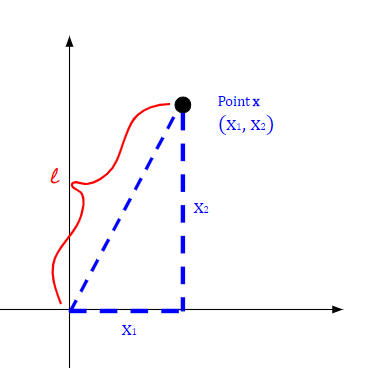
\includegraphics[scale=0.9]{assets/v_norm.png}
\end{center}
For a point \[\x = (x_1, x_2),\] we can define the \emph{2-norm} of a vector to be \[||\x||_2 = \sqrt{x_{1}^{2} + x_{2}^{2}}.\]

\begin{definition}{Vector Norm}{}
    A \textbf{norm} of a vector (i.e., a \textbf{vector norm}) $\x \in \R^n$ is a real number $||\x||$ that is assigned to $\x$. For all $\x, \y \in \R^n$ and all $c \in \R$, the following properties are satisfied: 
    \begin{enumerate}
        \item \underline{Positive Definite Property:} $||\x|| > 0$ for $\x \neq 0$ and $||\0|| = 0$. 
        \item \underline{Absolute Homogeneity:} $||c\x|| = |c| \cdot ||\x||$. 
        \item \underline{Triangle Inequality:} $||\x + \y|| \leq ||\x|| + ||\y||$. 
    \end{enumerate}
\end{definition}
\textbf{Remark:} With regards to the third property, consider \begin{center}
    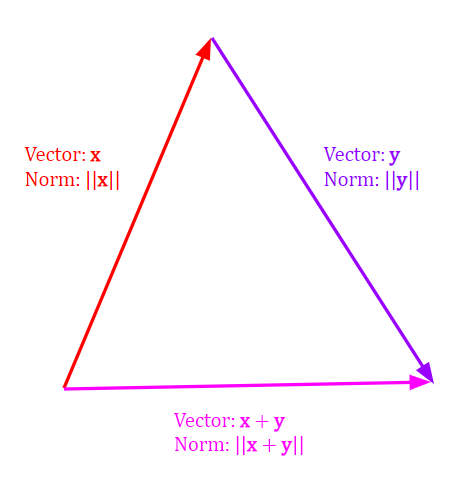
\includegraphics[scale=0.6]{assets/tri_inequality.png}
\end{center}
Note that $||\x + \y|| = ||\x|| + ||\y||$ if $\x$ and $\y$ points at the same direction.

\subsubsection{Common Norms}
There are some common norms that we've seen before. As implied, they all satisfy the properties above. 
\begin{itemize}
    \item For $p \geq 1$, we define 
    \[||\x||_p = \sqrt[p]{|x_1|^p + |x_2|^p + \hdots + |x_n|^p}.\]
    Note that some special cases are 
    \[||\x||_2 = \sqrt{x_1^2 + x_2^2 + \hdots + x_n^2}\]
    and 
    \[||\x||_1 = |x_1| + |x_2| + \hdots + |x_n| = \sum_{i = 1}^{n} |x_i|.\]

    \item The infinite norm is defined to be \[||\x||_{\infty} = \max_{i = 1, 2, \hdots, n} |x_i|.\] It should be noted that \[\lim_{p \mapsto \infty} ||\x||_p = ||\x||_{\infty}.\]
\end{itemize}

\begin{mdframed}
    (Exercise.) Consider the vector, \[\vv = \begin{bmatrix}
        4 \\ 8 \\ 6
    \end{bmatrix}.\]

    \begin{itemize}
        \item Compute $||\vv||_1$.
        \begin{mdframed}
            \[||\vv||_1 = |4| + |8| + |6| = 18.\]
        \end{mdframed}

        \item Compute $||\vv||_2$.
        \begin{mdframed}
            \[||\vv||_2 = \sqrt{4^2 + 8^2 + 6^2} = \sqrt{116}.\]
        \end{mdframed}

        \item Compute $||\vv||_\infty$. 
        \begin{mdframed}
            \[||\vv||_\infty = \max_{i = 1, 2, 3} |v_i| = \max\{|4|, |8|, |6|\} = 8.\]
        \end{mdframed}
    \end{itemize}
\end{mdframed}

\subsection{Matrix Norms}
We now want to consider norms for a matrix $A \in \R^{n \times n}$. There are two ways we can interpret matrix norms.
\begin{enumerate}
    \item Interpret matrix as a vector. For example, suppose we have \[A = \begin{bmatrix}
        -1 & 0 & 5 \\ 8 & 2 & 7 \\ -3 & 1 & 0
    \end{bmatrix}.\] Then, we can ``convert'' this matrix to a vector like so: \[\vv = \begin{bmatrix}
        -1 \\ 0 \\ 5 \\ 8 \\ 2 \\ 7 \\ -3 \\ 1 \\ 0
    \end{bmatrix}.\] Here, $\vv \in \R^9$. Notice how the first column of $A$ is the top three elements in $\vv$, the second column of $A$ is the middle three elements of $\vv$, and the last column of $A$ is the bottom three elements of $\vv$. 

    \item We can also define the matrix as a linear operator. That is, for a function $L: \R^n \mapsto \R^n$, we have \[L(\x) = A\x.\]
\end{enumerate}

\subsubsection{General Definition of Matrix Norms}
\begin{definition}{Matrix Norm}{}
    A \textbf{matrix norm} assigns a real number $||A||$ to a matrix $A$. This should satisfy the following conditions for all $A, B \in \R^{n \times n}$ and $c \in \R$. 
    \begin{enumerate}
        \item $||A|| > 0$ if $A \neq 0$, and $||0|| = 0$. 
        \item $||cA|| = |c| \cdot ||A||$. 
        \item $||A + B|| \leq ||A|| + ||B||$.
        \item Submultiplicity: $||AB|| \leq ||A|| \cdot ||B||$.  
    \end{enumerate}
\end{definition}
\textbf{Remark:} Regarding submultiplicity, for any $\x, \y \in \R^n$, we have \[|\cyclic{x, y}| \leq ||\x||_2 ||y||_2,\] known as the Cauchy Schwarz inequality. 

\subsubsection{Vector Viewpoint}
Going back to the vector viewpoint, let's suppose we have \[A = \begin{bmatrix}
    a_{11} & a_{12} & \hdots & a_{1n} \\ 
    a_{21} & a_{22} & \hdots & a_{2n} \\ 
    \vdots & \vdots & \ddots & \vdots \\ 
    a_{n1} & a_{n2} & \hdots & a_{nn}
\end{bmatrix}.\] Then, 
\[\vv = \begin{bmatrix}
    a_{11} \\ a_{21} \\ \vdots \\ a_{n1} \\ a_{12} \\ a_{22} \\ \vdots \\ a_{n2} \\ \vdots \\ a_{1n} \\ a_{2n} \\ \vdots \\ a_{nn}
\end{bmatrix}.\]

The Frobenius norm of $A$ is defined by 
\[||A||_F = ||\vv||_2 = \left(\sum_{i = 1}^{n} \sum_{j = 1}^{n} |a_{ij}|^2\right)^{\frac{1}{2}}.\]

\subsubsection{Matrix Norm}
Matrix $p$-norms are defined as follows: 
\[||A||_p = \max_{\substack{\x \in \R^n \\ \x \neq \0}} \frac{||A\x||_p}{||\x||_p}.\]
This measures the \emph{maximum stretch} the linear function $L(\x) = A\x$ can do to a vector (normalized by the length of the vector).

\bigskip 

Some of the most important matrix $p$-norms are 
\begin{itemize}
    \item For $p = 1$, \[||A||_1 = \max_{\x \neq \0} \frac{||A\x||_1}{||\x||_1} = \max_{j = 1, 2, \hdots, n} \sum_{i = 1}^{n} |a_{ij}|,\] the maximum $L_1$-norm of each column.
    \item For $p = \infty$, \[||A||_\infty = \max_{\x \neq \0} \frac{||A\x||_\infty}{||\x||_\infty} = \max_{i = 1, 2, \hdots, n} \sum_{j = 1}^{n} |a_{ij}|,\] the maximum $L_1$-norm of each row.
    \item For $p = 2$: \[||A||_2 = \max_{\x \neq \0} \frac{||A\x||_2}{||\x||_2} = \sigma_1,\] the largest\footnote{This is related to SVD, which we will learn later.} singular value of matrix $A$.
\end{itemize}
\textbf{Remark:} Don't confuse $||A||_2$ and $||A||_F$. They are very different! Specifically, 
\[||A||_2 = \max_{\x \neq \0} \frac{||A\x||_2}{||\x||_2}\]
while 
\[||A||_F = ||\vv||_2 = \left(\sum_{i, j} (a_{ij})^2\right)^{\frac{1}{2}}.\]

\begin{mdframed}
    (Exercise.) Consider the following matrix 
    \[A = \begin{bmatrix}
        4 & 8 & 6 \\ 
        8 & 17 & 10 \\ 
        6 & 10 & 29
    \end{bmatrix}.\]

    \begin{itemize}
        \item Compute $||A||_F$.
        \begin{mdframed}
            \[||A||_F = \sqrt{4^2 + 8^2 + 6^2 + 8^2 + 17^2 + 10^2 + 6^2 + 10^2 + 29^2} = \sqrt{1546}.\]
        \end{mdframed}

        \item Compute $||A||_1$.
        \begin{mdframed}
            We consider the sum of the absolute value of the entries in each column. 
            \begin{itemize}
                \item For the first column, we know that 
                \[\sum_{i = 1}^{3} |a_{i1}| = |4| + |8| + |6| = 18.\]
                \item For the second column, 
                \[\sum_{i = 1}^{3} |a_{i2}| = |8| + |17| + |10| = 35.\]
                \item For the third column, 
                \[\sum_{i = 1}^{3} |a_{i3}| = |6| + |10| + |29| = 45.\]
            \end{itemize}
            Therefore, \[||A||_1 = \max\{18, 35, 45\} = 45.\]
        \end{mdframed}

        \item Compute $||A||_\infty$. 
        \begin{mdframed}
            We consider the sum of the absolute value of the entries in each row. 
            \begin{itemize}
                \item For the first row, 
                \[\sum_{j = 1}^{3} |a_{1j}| = |4| + |8| + |6| = 18.\]
                \item For the second row, 
                \[\sum_{j = 1}^{3} |a_{2j}| = |8| + |17| + |10| = 35.\]
                \item For the third row, 
                \[\sum_{j = 1}^{3} |a_{3j}| = |6| + |10| + |29| = 45.\]
            \end{itemize}
            Therefore, \[||A||_\infty = \max\{18, 35, 45\} = 45.\]
        \end{mdframed}
    \end{itemize}
\end{mdframed}

\section{The Discrete Least Squares Problem (Section 3.1)}
Given points $(t_1, y_1), (t_2, y_2), \hdots, (t_n, y_n)$, we want to find an \emph{approximate function} to fit those points; that is, \[p(t_i) = y_i\] for $i = 1, 2, \hdots, n$. For example, suppose we want to find \[p(t) = a_0 + a_1 t\] or \[p(t) = a_0 + a_1 t + a_2 t^2.\] The idea is that we're just trying to find the \emph{line of best fit} (a line with the smallest margin of error). We're not trying to find a line that passes through all the points, just the one of best fit.
\begin{center}
    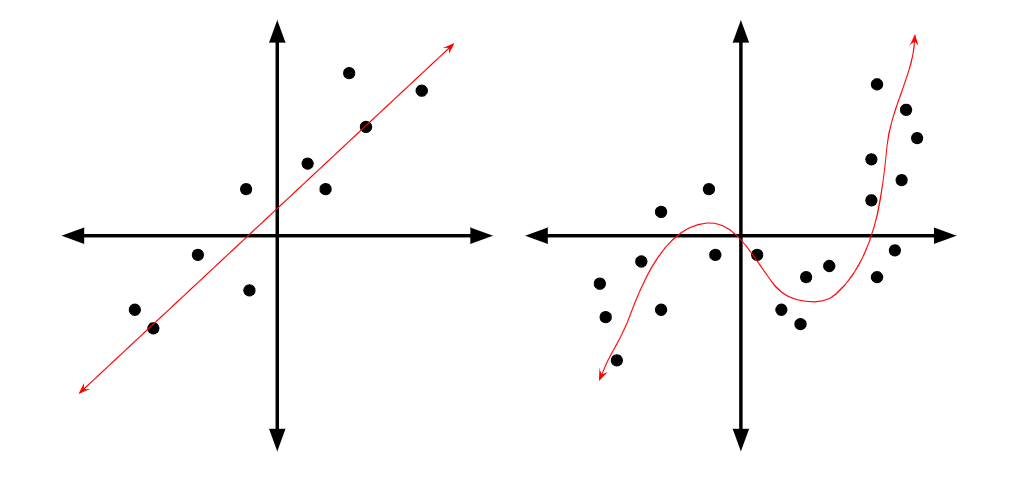
\includegraphics[scale=0.7]{assets/line_best_fit.png}
\end{center}
The error, as mentioned, is defined by $r_i = y_i - p(t_i)$, where $y_i$ is the exact value and $p(t_i)$ is the value of the function (the estimate). Then, the $r_i$'s generate a vector known as the \textbf{residual} vector.

\subsection{Problem Statement}
Our goal is to find a $p(t) = a_0 + a_1 t$ such that $r \in \R^a$ is as small as possible. Hence, it turns into finding $a_0, a_1$ to minimize $||r||_2$. 

\subsubsection{Matrix Notation}
Let's begin by converting 
\[r_i = y_i - p(t_i) = y_i - (a_0 + a_1 t_i) = y_i - a_0 - a_1 t_i \quad i = 1, 2, \hdots, n\]
into matrix notation. This gives us 
\[\underbrace{\begin{bmatrix}
    r_1 \\ r_2 \\ \vdots \\ r_n
\end{bmatrix}}_{\rr \in \R^n} = \begin{bmatrix}
    y_1 - a_0 - a_1 t_1 \\ 
    y_2 - a_0 - a_1 t_2 \\ 
    \vdots \\ 
    y_n - a_0 - a_1 t_n
\end{bmatrix} = \begin{bmatrix}
    y_1 \\ y_2 \\ \vdots \\ y_n
\end{bmatrix} \begin{bmatrix}
    a_0 + a_1 t_1 \\ 
    a_0 + a_1 t_2 \\
    \vdots \\ 
    a_0 + a_1 t_n
\end{bmatrix} = \underbrace{\begin{bmatrix}
    y_1 \\ y_2 \\ \vdots \\ y_n
\end{bmatrix}}_{\y \in \R^n} - \underbrace{\begin{bmatrix}
    1 & t_1 \\ 
    1 & t_2 \\ 
    \vdots & \vdots \\ 
    1 & t_n
\end{bmatrix}}_{A \in \R^{n \times m}} \underbrace{\begin{bmatrix}
    a_0 \\ a_1
\end{bmatrix}}_{\x \in \R^{m}}\]
So, with the above matrix notation, also represented by 
\[\rr = \y - A\x,\]
the goal is to find an $\x \in \R^m$ such that $||\rr||_2$ is minimized. Essentially, 
\[\min_{x \in \R^m} ||\rr||_2 = \min_{x \in \R^m} ||\y - A\x||_2.\] Here, 
\begin{itemize}
    \item $n$ is the number of datapoints, and
    \item $m$ is the number of unknowns from the function. 
\end{itemize} 
\textbf{Remarks:}
\begin{itemize}
    \item $A$ is not squared.
    \item $n > m$.
\end{itemize} 
There will be no solutions\footnote{$A$ has more rows than columns.} to $A\x = \y$. Instead, we want to find $\x$ that minimizes the overall error.

\subsection{Other Basis Functions}
Instead of linear functions $p(t) = a_0 + a_1 t$, we an try other types of functions. For example, consider polynomials, or \[p(t) = a_0 + a_1 t + a_2 t^2 + \hdots + a_k t^k = \sum_{i = 0}^{k} a_i t^i.\] Here, $t^0 = 1$ and we have $(k + 1)$ unknowns. The matrix formulation is given by

\[\underbrace{\begin{bmatrix}
    r_1 \\ r_2 \\ \vdots \\ r_n
\end{bmatrix}}_{r \in \R^n} = \begin{bmatrix}
    y_1 - p(t_1) \\ 
    y_2 - p(t_2) \\ 
    \vdots \\ 
    y_n - p(t_n)
\end{bmatrix} = \begin{bmatrix}
    y_1 \\ y_2 \\ \vdots \\ y_n
\end{bmatrix} - \begin{bmatrix}
    p(t_1) \\ p(t_2) \\ \vdots \\ p(t_n)
\end{bmatrix} = \underbrace{\begin{bmatrix}
    y_1 \\ y_2 \\ \vdots \\ y_n
\end{bmatrix}}_{\y \in \R^n} - \underbrace{\begin{bmatrix}
    1 & t_1 & t_1^2 & \hdots & t_1^k \\ 
    1 & t_2 & t_2^2 & \hdots & t_2^k \\ 
    \vdots & \vdots & \vdots & \ddots & \vdots \\ 
    1 & t_n & t_n^2 & \hdots & t_n^k
\end{bmatrix}}_{A \in \R^{nn \times (k + 1)}} \underbrace{\begin{bmatrix}
    a_0 \\ a_1 \\ \vdots \\ a_k
\end{bmatrix}}_{\x \in \R^{k + 1}}.\]

Here, $\rr = \y - A\x$ is called the \emph{residual}. To solve this, we will use the QR decomposition. 

\subsection{QR Decomposition}
In essence, QR decomposition states that we can decompose a matrix $A$ into two matrices, $Q$ and $R$, such that 
\[A = QR,\]
where $Q$ is orthogonal and $R$ is upper-triangular. 

\subsubsection{A Brief Review}
\begin{definition}{Orthogonal Matrix}{}
    $Q \in \R^{n \times n}$ is called \textbf{orthogonal} if $Q^T = Q^{-1}$, i.e., $Q^T Q = QQ^T = I$. 
\end{definition}

\begin{mdframed}
    (Example.) Consider the rotations in $\R^n$. Note that 
    \[Q = \begin{bmatrix}
        \cos\theta & -\sin\theta \\ 
        \sin\theta & \cos\theta
    \end{bmatrix} \quad Q^T = \begin{bmatrix}
        \cos\theta & \sin\theta \\ 
        -\sin\theta & \cos\theta 
    \end{bmatrix}.\]
    It follows that \[QQ^T = \begin{bmatrix}
        1 & 0 \\ 0 & 1
    \end{bmatrix} = I.\]
\end{mdframed}

\begin{theorem}{}{}
    If $Q \in \R^{n \times n}$ is an orthogonal matrix, then 
    \begin{enumerate}
        \item $\cyclic{Q\x, Q\y} = \cyclic{\x, \y}$. 
        \item $||Q\x||_2 = ||\x||_2$.
    \end{enumerate}    
\end{theorem}
It might be useful to consider this visualization: 
\begin{center}
    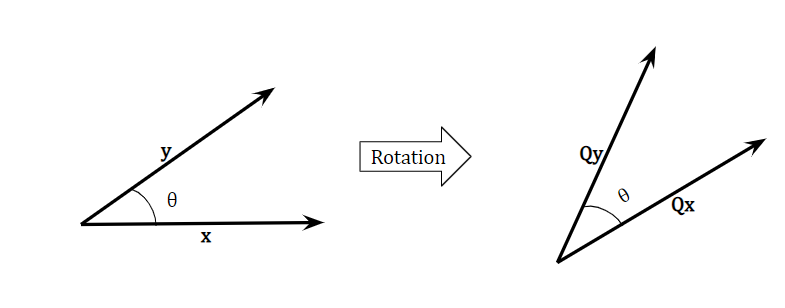
\includegraphics[scale=0.8]{assets/angle_orth.png}
\end{center}

\begin{proof}
    We'll prove each part. 
    \begin{enumerate}
        \item $\cyclic{Q\x, Q\y} = (Q\x)^T Q\y = \x^T Q^T Q \y = \x^T \y = \cyclic{\x, \y}$. 
        \item $||Q\x||_2 = \sqrt{\cyclic{Q\x, Q\y}} = \sqrt{\cyclic{\x, \x}} = ||\x||_2$. 
    \end{enumerate}
    Thus, we're done.
\end{proof}


\section{Solutions to the Discrete Least Squares Problem (Section 3.3)}
In the previous section, we learned how to construct a Least Squares Problem given a set of points. The idea was to find a function such that the residual was minimized. We talked briefly about using QR decomposition and how it could be used to solve this problem. Now, we'll talk more about using QR decomposition. 

\begin{theorem}{Full QR Decomposition}{}
    Let $A \in \R^{n \times m}$ such that $n \geq m$. Then, there exists an orthogonal $Q \in \R^{n \times n}$ and $R \in \R^{n \times m}$ with 
    \[R = \begin{bmatrix}
        r_{11} & r_{12} & \hdots & r_{1m} \\ 
        0 & r_{22} & \hdots & r_{2m} \\
        0 & 0 & \hdots & r_{3m} \\ 
        \vdots & \vdots & \ddots & \vdots \\ 
        0 & 0 & \hdots & r_{nm} \\ 
        0 & 0 & \hdots & 0 \\ 
        0 & 0 & \hdots & 0 \\ 
        0 & 0 & \hdots & 0 \\ 
        \vdots & \vdots & \ddots & 0 \\ 
        0 & 0 & \hdots & 0
    \end{bmatrix} = \begin{bmatrix}
        \hat{R} \\ 0
    \end{bmatrix},\]
    with $\hat{R} \in \R^{m \times m}$ being an upper-triangular matrix and the 0 being the zero-matrix, such that \[A = QR.\]
\end{theorem}
\textbf{Remark:} If $A$ has full rank ($\text{rank}(A) = \min\{n, m\} = m$) and we choose $n_i > 0$, then the reduced QR is unique. 

\subsection{Purpose of QR}
One of the main purposes of the QR decomposition is to solve the Least Squares Problem. Note that methods like LU and PLU decompositions are not useful because the matrix we're working with is a tall matrix ($n \geq m$). 

\bigskip 

Now, that being said, there are two cases to consider. 
\begin{enumerate}
    \item If $A$ is a square matrix and invertible, then it still has a QR decomposition. Note that 
    \begin{equation*}
        \begin{aligned}
            A\x = \y &\implies QR\x = \y \\ 
                &\implies Q^T Q R \x = Q^T \y \\ 
                &\implies R\x = Q^T \y. 
        \end{aligned}
    \end{equation*}

    \item Otherwise, recall that \[\min_{\x \in \R^m} ||\y - A\x||_{2}^{2}\] with $A \in \R^{n \times m}$ and $n \geq m$. Assume that $A$ has a QR decomposition such that \[A = QR,\] we want to compute \[||\y - A\x||_{2}^{2}.\] Notice that
    \begin{equation*}
        \begin{aligned}
            ||\y - A\x||_2^2 &= ||\y - QR\x||_2^2 \\ 
                &= ||I\y - QR\x||_2^2 \\ 
                &= ||QQ^T \y - QR\x||_2^2 \\ 
                &= ||Q(Q^T \y - R\x)||_2^2 \\ 
                &= ||Q^T \y - R\x||_2^2 && Q \text{ is orthogonal, so} ||Q\x||_2^2 = ||\x||_2^2 \\ 
                &= \left|\left| \begin{bmatrix}
                    \hat{c} \\ d
                \end{bmatrix} - \begin{bmatrix}
                    \hat{R} \\ 0
                \end{bmatrix} \x \right|\right|_2^2 \\ 
                &= \left|\left| \begin{bmatrix}
                    \hat{c} - \hat{R}\x \\ 
                    d 
                \end{bmatrix} \right|\right|_2^2 \\ 
                &= ||\hat{c} - \hat{R}\x||_2^2 + ||d||_2^2
        \end{aligned}
    \end{equation*}

    Recall that we rewrote $R$ so that \[R = \begin{bmatrix}
        \hat{R} \\ \0
    \end{bmatrix}.\] We can rewrite $Q^T \y$ so that \[Q^T \y = \begin{bmatrix}
        \hat{c} \\ d
    \end{bmatrix},\] where $\hat{c}$ and $d$ are vectors of length $m$.  
\end{enumerate}
With this in mind, we have 
\[\min_{\x \in \R^m} ||\y - A\x||_2^2 = \min_{\x \in \R^m} ||\hat{c} - \hat{R}\x||_2^2 + ||d||_2^2.\]
Here, $\min_{\x \in \R^m} ||\hat{c} - \hat{R}\x||_2^2$ is the solution to $\hat{R}\x = \hat{c}$, with $\hat{c} = Q^T \y(1 : m)$ and $\hat{R} = R(1:m, 1:m)$ and $A = QR$ is a QR decomposition. Additionally, $\hat{R}\x = \hat{c}$ has a unique solution $\x$, assuming $\text{rank}(A) = m$ and $\hat{c} - \hat{R}\x = \0$. The norm of the residual is $||d||_2$. 


\begin{mdframed}
    (Example.) Suppose we have $\min_{\x \in \R^m} ||\y - A\x||_2^2$ with \[A = \begin{bmatrix}
        -1 & -1 & 1 \\ 
        1 & 3 & 3 \\ 
        -1 & -1 & 5 \\ 
        1 & 3 & 7
    \end{bmatrix}\] and \[\y = \begin{bmatrix}
        1 \\ 0 \\ -1 \\ 2
    \end{bmatrix}\] and want to find $\x$ by using QR. Because we haven't talked about how to do the QR decomposition, we'll give $Q$ and $R$ now: 
    \begin{equation*}
        \begin{aligned}
            \underbrace{\begin{bmatrix}
                -1 & -1 & 1 \\ 
                1 & 3 & 3 \\ 
                -1 & -1 & 5 \\ 
                1 & 3 & 7
            \end{bmatrix}}_{A \in \R^{4 \times 4}} &= \frac{1}{2} \underbrace{\begin{bmatrix}
                -1 & 1 & -1 & 1 \\ 
                1 & 1 & -1 & -1 \\ 
                -1 & 1 & 1 & -1 \\ 
                1 & 1 & 1 & 1
            \end{bmatrix}}_{Q \in \R^{4 \times 4}} \underbrace{\begin{bmatrix}
                2 & 4 & 2 \\ 
                0 & 2 & 8 \\ 
                0 & 0 & 4 \\ 
                0 & 0 & 0
            \end{bmatrix}}_{R \in \R^{4 \times 3}} \\ 
                &= \begin{bmatrix}
                    -\frac{1}{2} & \frac{1}{2} & -\frac{1}{2} & \frac{1}{2} \\ 
                    \frac{1}{2} & \frac{1}{2} & -\frac{1}{2} & -\frac{1}{2} \\ 
                    -\frac{1}{2} & \frac{1}{2} & \frac{1}{2} & -\frac{1}{2} \\ 
                    \frac{1}{2} & \frac{1}{2} & \frac{1}{2} & \frac{1}{2}
                \end{bmatrix} \begin{bmatrix}
                    2 & 4 & 2 \\ 
                    0 & 2 & 8 \\ 
                    0 & 0 & 4 \\ 
                    0 & 0 & 0
                \end{bmatrix}
        \end{aligned}
    \end{equation*}
    Note that\footnote{Recall that $\hat{R} = R(1:m, 1:m)$. In other words, we take the first $m$ rows and columns from $R$.} \[\hat{R} = \begin{bmatrix}
        2 & 4 & 2 \\ 
        0 & 2 & 8 \\ 
        0 & 0 & 4
    \end{bmatrix}.\] Additionally, note that \[Q^T \y = \begin{bmatrix}
        1 \\ 1 \\ 0 \\ 2
    \end{bmatrix}\] so it follows that \[\hat{c} = \begin{bmatrix}
        1 \\ 1 \\ 0
    \end{bmatrix}.\] Finally, $d = \begin{bmatrix}
        2
    \end{bmatrix} = 2$ (note that $d$ is a vector of the remaining entries after $\hat{c}$). Now, we can solve \[\hat{R}\x = \hat{c}.\] In particular,
    \[\begin{bmatrix}
        2 & 4 & 2 \\ 
        0 & 2 & 8 \\ 
        0 & 0 & 4
    \end{bmatrix} \begin{bmatrix}
        x_1 \\ x_2 \\ x_3
    \end{bmatrix} = \begin{bmatrix}
        1 \\ 1 \\ 0
    \end{bmatrix}.\] This gives us \[\x = \begin{bmatrix}
        -\frac{1}{2} \\ \frac{1}{2} \\ 0
    \end{bmatrix}.\]
    The norm of the residual is $||d||_2 = |2| = 2$. 
\end{mdframed}



\section{Projectors \& Reflectors (Section 3.2)}
In this section, we'll talk about projectors and reflectors, something that's important for QR decomposition.

\subsection{Projectors}
\begin{definition}{Projector}{}
    A \textbf{projector} is a matrix $P$ with \[P^2 = P.\] 
\end{definition}

\begin{definition}{Orthoprojector}{}
    If $P$ is a projector and also symmetric (i.e., $P = P^T$), then $P$ is called an \textbf{orthoprojector}.
\end{definition}

\begin{mdframed}
    (Example.) Suppose $\u \in \R^n$ is a unit vector (i.e., $||\u||_2 = 1$). Then, $P = \u \cdot \u^T$ is an orthoprojector. That is, 
    \[P = \begin{bmatrix}
        u_1 \\ u_2 \\ \vdots \\ u_n
    \end{bmatrix} \begin{bmatrix}
        u_1 & u_2 & \hdots & u_n
    \end{bmatrix} = \begin{bmatrix}
        u_1^2 & u_1 u_2 & \hdots & u_1 u_n \\ 
        u_2 u_1 & u_2^2 & \hdots & u_2 u_n \\ 
        \vdots & \vdots & \ddots & \vdots \\ 
        u_n u_1 & u_n u_1 & \hdots & u_n^2 
    \end{bmatrix}.\]
    To see why $P$ here is an orthoprojector, we'll show that it satisfies some properties. 
    \begin{enumerate}
        \item Definition of a projector.
        \[P^2 = P \cdot P = (\u \cdot \u^T) (\u \cdot \u^T) = \u (\underbrace{\u^T \u}_{1}) \u^T = \u \u^T = P.\]

        \item Definition of an orthoprojector.
        \[P^T = (\u \u^T)^T = (\u^T)^T \u^T = \u\u^T = P.\]
    \end{enumerate}
    There are some additional properties to know for this case. 
    \begin{itemize}
        \item $P\u = \u$:
        \[P\u = (\u\u^T)\u = \u(\underbrace{\u^T \u}_{1}) = \u.\]

        \item If $\vv \perp \u$ (i.e., $\cyclic{\vv, \u} = 0$), then $P\vv = \0$. 
        \[P\vv = (\u\u^T)\vv = \u(\underbrace{\u^T\vv}_{0}) = \0.\]
    \end{itemize}
\end{mdframed}
\textbf{Remarks:} 
\begin{itemize}
    \item Note that if $\u \in \R^{n \times 1}$, then $\u^T \in \R^{1 \times n}$ and so $P$ will be an $n \times n$ matrix.
    \item Note that $\u \u^T \neq \u^T \u$. In particular, $\u \u^T$ is an $n \times n$ matrix while $\u^T \u = \cyclic{\u, \u} = ||\u||_{2}^{2}$. 
\end{itemize}

\subsection{Reflectors}
Reflectors are built by \emph{projectors}.

\begin{definition}{Reflector}{}
    For a unit vector $\u \in \R^n$ (i.e., $||\u||_2 = 1$), $Q = I - 2\u \u^T$ is called a (householder) \textbf{reflector}. 
\end{definition}
\textbf{Remarks:} 
\begin{itemize}
    \item We can rewrite the above with $Q = I - 2P$, where $P = \u \u^T$ is a projector. 
    \item If $\u$ doesn't have unit norm, we can normalize it,
    \[\frac{\u}{||\u||_2},\]
    so that $\left|\left| \frac{\u}{||\u||_2} \right|\right|_2 = \frac{1}{||\u||_2} ||\u||_2 = 1$ (note that $||\u||_2$ is a scalar.) In this sense, we can write 
    \[Q = I - 2 \frac{\u}{||\u||_2} \frac{\u^T}{||\u||_2} = I - 2 \frac{\u\u^T}{||\u||_2^2}.\]
\end{itemize}
There are some properties of $Q = I - 2 \u\u^T$ (where $\u$ is a unit vector) to know.
\begin{enumerate}
    \item $Q\u = -\u$. 
    \[Q\u = (I - 2\u\u^T)\u = \u - 2\u\u^T\u = \u - 2\u = -\u.\]

    \item $Q\vv = \vv$ such that $\vv \perp \u$.
    \[Q\vv = (I - 2\u\u^T)\vv = \vv - 2\u\underbrace{\u^T\vv}_{\0} = \vv.\]

    \item $Q^T = Q$. 
    \[Q^T = (I - 2\u\u^T)^T = (I - 2P)^T = I - 2P^T = I - 2P = Q.\]
    Here, note that $I^T = I$. Additionally, note that $P^T = P$.

    \item $\underbrace{Q^T = Q^{-1}}_{\text{Orthogonal}}$ and $Q = Q^{-1}$ and $Q^T Q = Q^2 = I$. 
    \[Q^2 = QQ = (I - 2P)(I - 2P) = I - 2P - 2P + 4P^2 = I - 4P - 4P^2 = I - 4P + 4P = I.\]
\end{enumerate}

\begin{lemma}{}{}
    For any $\x \in \R^n$ and $\y \in \R^n$ such that \[\y = \begin{bmatrix}
        ||\x||_2 & 0 & 0 & \hdots & 0
    \end{bmatrix}^T,\]
    define $\vv = \x - \y$ and $\u = \frac{\vv}{||\vv||_2}$. Then, 
    \[Q = I - 2\u\u^T\] is a reflector satisfying $Q\x = \y$. 
\end{lemma}
\textbf{Remarks:} 
\begin{itemize}
    \item If $\x = \y$, then $Q = I$.
    \item Alternatively, if $\e_1 = \begin{bmatrix}
        1 & 0 & 0 & \hdots & 0
    \end{bmatrix}^T$, then 
    \[\y = ||\x||_2 \e_1.\] It should be noted that $\e_2 = \begin{bmatrix}
        0 & 1 & 0 & \hdots & 0
    \end{bmatrix}$ and $\e_n = \begin{bmatrix}
        0 & 0 & 0 & \hdots & 1
    \end{bmatrix}$. 
\end{itemize} 

\subsection{QR Decomposition (For the 3rd Time)}
We will talk about reduced QR later; for now, we will focus on full QR. The idea is that, with QR, we'll do something like 
\[Q_n \hdots Q_2 Q_1 A \mapsto R.\]
The idea is that, starting from $A$, we can multiply the reflectors multiple times until we end up with $R$, which is an upper-triangular matrix. This is analogous to LU decomposition, where we did 
\[L_n \hdots L_2 L_1 A \mapsto U.\]

Now, for QR decomposition, given $A \in \R^{n \times m}$ (our ``tall'' matrix), we want to find $QR$. We can rewrite $A$ in column form,
\[A = \begin{bmatrix}
    c_1 & c_2 & c_3 & \hdots & c_i & \hdots & c_m
\end{bmatrix},\] 
where $c_i$ is the $i$th column for $i = 1, 2, \hdots, m$. Recall that we want to derive $R$; that is, we want an upper-triangular matrix. So, starting from the first column, we want to make all the entries under $a_{11}$ 0. We can use a reflector mapping $Q_1$ to map the column,
\[c_1 \mapsto ||c_1|| \e_1\]
where $\e_1 \in \R^n$, so that we end up with
\[Q_1 A = \begin{bmatrix}
    ||c_1|| & * & * & \hdots & * \\ 
    0 & * & * & \hdots & * \\ 
    \vdots & \vdots & \vdots & \ddots & \vdots \\ 
    0 & * & * & \hdots & *
\end{bmatrix} = \begin{bmatrix}
    ||c_1|| & * & * & \hdots & * \\ 
    0 & \underline{*} & \underline{*} & \hdots & \underline{*} \\ 
    \vdots & \vdots & \vdots & \ddots & \vdots \\ 
    0 & \underline{*} & \underline{*} & \hdots & \underline{*}
\end{bmatrix}.\]
From the above matrix, we can represent the underlined stars as a new matrix: \[\tilde{A} = \begin{bmatrix}
    \underline{*} & \underline{*} & \hdots & \underline{*} \\ 
    \vdots & \vdots & \ddots & \vdots \\ 
    \underline{*} & \underline{*} & \hdots & \underline{*}
\end{bmatrix} \in \R^{(n - 1) \times (m - 1)}.\]
So, if we have 
\[\tilde{A} = \begin{bmatrix}
    \tilde{c_2} & \tilde{c_3} & \hdots & \tilde{c_m}
\end{bmatrix},\] we want to define a reflector mapping \[\tilde{Q_2}: \tilde{c_2} \mapsto ||\tilde{c_2}|| \tilde{e_1}\] where $\tilde{e_1} \in \R^{n - 1}$. Now, define \[Q_2 = \begin{bmatrix}
    1 & 0 \\ 
    0 & \tilde{Q_2}
\end{bmatrix}\] so that \[Q_2 Q_1 A = \begin{bmatrix}
    ||c_1|| & * & * & \hdots & * \\ 
    0 & ||\tilde{c_2}|| & * & \hdots & * \\ 
    0 & 0 & * & \hdots & * \\
    \vdots & \vdots & \vdots & \ddots & \vdots \\ 
    0 & 0 & * & \hdots & *
\end{bmatrix} = \begin{bmatrix}
    ||c_1|| & * & * & \hdots & * \\ 
    0 & ||\tilde{c_2}|| & * & \hdots & * \\ 
    0 & 0 & \underline{*} & \hdots & \underline{*} \\
    \vdots & \vdots & \vdots & \ddots & \vdots \\ 
    0 & 0 & \underline{*} & \hdots & \underline{*}
\end{bmatrix}.\] From this, we can define \[B = \begin{bmatrix}
    \underline{*} & \hdots & \underline{*} \\ 
    \vdots & \ddots & \vdots \\ 
    \underline{*} & \hdots & \underline{*}
\end{bmatrix}.\] Continuing this process, we should eventually end up with \[Q_m \hdots Q_1 A = \begin{bmatrix}
    ||c_1|| & * & * & \hdots & * \\ 
    0       & ||\tilde{c_2}|| & * & \hdots & * \\ 
    0       & 0               & ||\tilde{c_3}|| & \hdots & * \\ 
    \vdots  & \vdots          & \vdots          & \ddots & * \\ 
    0       & 0               & 0               & \hdots & ||\tilde{c_m}|| \\ 
    \vdots  & \vdots          & \vdots          & \vdots & \vdots \\ 
    0 & 0 & 0 & 0 & 0
\end{bmatrix} = R.\]
Note that $\tilde{Q}A = R \implies A = QR$. Then, the question becomes: how do we define $Q$? We can define $Q$ as\footnote{Recall that $\tilde{Q}$ is orthogonal.} \[Q = \tilde{Q}^{-1} = \tilde{Q}^{T}.\] 
\textbf{Remarks:}
\begin{itemize}
    \item The product of orthogonal matrices is \textbf{orthogonal}.
    \item The inverse of orthogonal matrices is \textbf{orthogonal}.
    \item Note that full QR is not unique.
\end{itemize}
Now, if $A$ has full rank and $r_{ii} > 0$ (the diagonal on the $R$), then the QR decomposition is unique. Note that 
\begin{itemize}
    \item If $A$ has full rank, then $A$ has $m$ linearly independent columns and $\text{rank}(A) = \min\{n, m\} = m$.
\end{itemize}


\section{Reduced QR (Section 3.4)}
Let's begin with an example from a few sections ago. Suppose we have the following \textbf{full QR decomposition}
\begin{equation*}
    \begin{aligned}
        \underbrace{\begin{bmatrix}
            -1 & -1 & 1 \\ 
            1 & 3 & 3 \\ 
            -1 & -1 & 5 \\ 
            1 & 3 & 7
        \end{bmatrix}}_{A \in \R^{4 \times 4}} &= \begin{bmatrix}
            -\frac{1}{2} & \frac{1}{2} & -\frac{1}{2} & \frac{1}{2} \\ 
            \frac{1}{2} & \frac{1}{2} & -\frac{1}{2} & -\frac{1}{2} \\ 
            -\frac{1}{2} & \frac{1}{2} & \frac{1}{2} & -\frac{1}{2} \\ 
            \frac{1}{2} & \frac{1}{2} & \frac{1}{2} & \frac{1}{2}
        \end{bmatrix} \begin{bmatrix}
            2 & 4 & 2 \\ 
            0 & 2 & 8 \\ 
            0 & 0 & 4 \\ 
            0 & 0 & 0
        \end{bmatrix} \\ 
            &= \frac{1}{2} \underbrace{\begin{bmatrix}
                -1 & 1 & -1 & 1 \\ 
                1 & 1 & -1 & -1 \\ 
                -1 & 1 & 1 & -1 \\ 
                1 & 1 & 1 & 1
            \end{bmatrix}}_{Q \in \R^{4 \times 4}} \underbrace{\begin{bmatrix}
                2 & 4 & 2 \\ 
                0 & 2 & 8 \\ 
                0 & 0 & 4 \\ 
                0 & 0 & 0
            \end{bmatrix}}_{R \in \R^{4 \times 3}}.
    \end{aligned}
\end{equation*}
Here, $Q$ is orthogonal and $R$ is a tall matrix. Let's look at $R$. Notice how the last row of $R$ are just 0's. In particular, the last column of the matrix $Q$ and the last row of $R$ yields 0's everywhere; it's not helpful. So, what if we throw away the last row of $R$ and corresponding columns of $Q$? This brings us to the topic of \textbf{reduced QR}. In particular,
\[\underbrace{\begin{bmatrix}
    -1 & -1 & 1 \\ 
    1 & 3 & 3 \\ 
    -1 & -1 & 5 \\ 
    1 & 3 & 7
\end{bmatrix}}_{A \in \R^{4 \times 4}} = \frac{1}{2} \underbrace{\begin{bmatrix}
    -1 & 1 & -1 \\ 
    1 & 1 & -1 \\ 
    -1 & 1 & 1 \\ 
    1 & 1 & 1
\end{bmatrix}}_{\hat{Q} \in \R^{4 \times 3}} \underbrace{\begin{bmatrix}
    2 & 4 & 2 \\ 
    0 & 2 & 8 \\ 
    0 & 0 & 4
\end{bmatrix}}_{\hat{R} \in \R^{3 \times 3}}.\]
\textbf{Remark:} $\hat{Q}$ is not a square matrix anymore; it's a tall matrix. The concept of orthogonal matrices does not make sense here anymore. Instead, note that $\hat{Q}$ is an \textbf{isometry}; 
\[\underbrace{\hat{Q}^T}_{3 \times 4} \underbrace{\hat{Q}}_{4 \times 3} = \underbrace{I}_{3 \times 3}.\]
(Compare this to orthogonal, where we have $Q^T Q = QQ^T = I$.)

\begin{theorem}{Reduced QR}{}
    Suppose $A \in \R^{n \times m}$ such that $n \geq m$. Then, there exists a $\hat{Q} \in \R^{n \times m}$ isometry and $\hat{R} \in \R^{m \times m}$ upper-triangular such that \[A = \hat{Q}\hat{R}.\]
\end{theorem}
\textbf{Remark:} The reduced QR decomposition is unique if $\text{rank}(A) = m$ and we choose $r_{ii} > 0$ (entry on diagonal of $\hat{R}$). 


\subsection{Orthonormal Set}
Before we talk about how to obtain the reduced QR decomposition, we first introduce orthonormal sets. 
\begin{definition}{Orthonormal Set}{}
    We say that\footnote{Note that $q_i$ is a \emph{vector}.}
    \[\{q_1, q_2, \hdots, q_m\}\]
    is called \textbf{orthonormal} if $\cyclic{q_i, q_j} = 0$ whenever $i \neq j$ and $\cyclic{q_i, q_i} = 1$.
\end{definition}
\textbf{Remark:} If $Q$ is orthogonal (isometry), then the columns are orthonormal. For example, if the set $\{e_1, e_2\}$ is orthonormal, then this might visually look like 
\begin{center}
    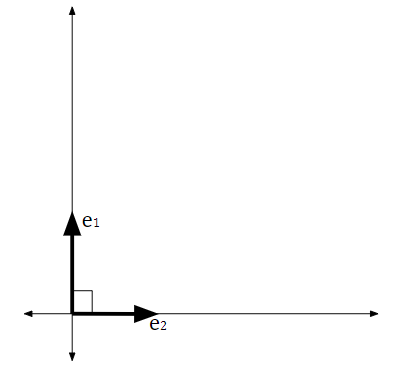
\includegraphics[scale=0.7]{assets/orthonormal.png}
\end{center}

\subsection{Gram-Schmidt}
With the idea of orthonormal sets in mind, the idea is to use the \textbf{Gram-Schmidt} algorithm to make the columns of $A$ into an orthonormal set $\{q_1, q_2, \hdots, q_m\}$. This represents $\hat{Q}$. 

\bigskip 

Notationally, assuming $A$ has full rank (i.e., linearly independent), we can say that \[\{a_1, a_2, \hdots, a_m\}\] represents the columns of $A$. 


\subsubsection{Classical Algorithm}
Given $A$, we want to find $\hat{Q}$ and $\hat{R}$ such that $A = \hat{Q}\hat{R}$. As mentioned above, we can write $A$ as a set of linearly independent columns, 
\[\begin{bmatrix}
    a_1, a_2, \hdots, a_m
\end{bmatrix}.\]
We can also write $\hat{Q}$ in the same way:
\[\begin{bmatrix}
    q_1, q_2, \hdots, q_m
\end{bmatrix}.\]
We can write $\hat{R}$ like so: 
\[\begin{bmatrix}
    r_{11} & r_{12} & \hdots & r_{1m} \\ 
    0 & r_{22} & \hdots & r_{2m} \\ 
    \vdots & \vdots & \ddots & \vdots \\ 
    0 & 0 & \hdots & r_{mm}
\end{bmatrix}.\]
Combining this, we end up with 
\[\begin{bmatrix}
    a_1, a_2, \hdots, a_m
\end{bmatrix} = \begin{bmatrix}
    q_1, q_2, \hdots, q_m
\end{bmatrix} \begin{bmatrix}
    r_{11} & r_{12} & \hdots & r_{1m} \\ 
    0 & r_{22} & \hdots & r_{2m} \\ 
    \vdots & \vdots & \ddots & \vdots \\ 
    0 & 0 & \hdots & r_{mm}
\end{bmatrix}.\]
Then, we note that 
\[a_1 = q_1 r_{11} \implies q_1 = \frac{a_1}{r_{11}} \implies r_{11} = ||a_1||_2.\]
\[a_2 = q_1 r_{12} + q_2 r_{22}.\]
\[a_3 = q_1 r_{13} + q_2 r_{23} + q_3 r_{33}.\]
Eventually, we'll end up with 
\[a_m = q_1 r_{1m} + q_2 r_{2m} + \hdots + q_m r_{mm}.\]
So, this is the basic idea: processing each column one at a time. Writing this out as steps, we have: 
\begin{enumerate}
    \item $r_{11} = ||a_1||_2$, $q_1 = \frac{a_1}{r_{11}} = \frac{a_1}{||a_1||_2}$. It follows that \[||q_1||_2 = 1.\]
    \item $a_2 = r_{12}q_1 + r_{22}q_2$. Then, we can multiply $q_1$ on both sides: 
    \begin{equation*}
        \begin{aligned}
            \cyclic{a_2, q_1} &= \cyclic{r_{12}q_1 + r_{22}q_2, q_1} \\ 
                &= r_{12}\underbrace{\cyclic{q_1, q_1}}_{1} + r_{22} \underbrace{\cyclic{q_2, q_1}}_{0} \\ 
                &= r_{12}.
        \end{aligned}
    \end{equation*}
    Note that we got the 0 and 1 from the properties of orthonormal sets. In any case, it follows that \[q_2 = \frac{a_2 - r_{12}q_1}{r_{22}}.\]
    Setting $r_{22} = ||a_2 - r_{12}q_1||_2$, it follows that $||q_2||_2 = 1$. 

    \item We start from $a_3$ and determine $q_3$ and $r_{13}$, $r_{23}$, and $r_{33}$. 
\end{enumerate}
Notice that we essentially keep going like this. Let's try to generalize this. The formula for $\hat{R}$ is given by 
\[\hat{R} = (r_{ji})\]
for $j < i$. Then, \[\hat{Q} = \begin{bmatrix}
    q_1 & q_2 & \hdots & q_m
\end{bmatrix}\] and we can get $A = \hat{Q} \hat{R}$. Remember that 
\[r_{12} = \cyclic{a_2, q_1}.\] Note that the 1 in $r$ index corresponds to the 1 in $q_1$ and the 2 in the $r$ index corresponds to the 2 in $a_2$. We also know that 
\[r_{22} = ||a_2 - r_{12}q_1||_2\] and 
\[q_2 = \frac{a_2 - r_{12}q_1}{r_{22}}.\]
Analogously, notice that 
\[r_{13} = \cyclic{a_3, q_1}\] and \[r_{23} = \cyclic{a_3, q_2}.\] We also know that \[a_{33} = ||a_3 - r_{13}q_1 - r_{23}q_2||_2\] and \[q_3 = \frac{a_3 - \sum_{j = 1}^{2} r_{j3} q_j}{r_{33}}.\] 
\underline{So, to conclude, we can generalize the formula:}
\[r_{ii} = \left|\left| a_{i} - \sum_{j = 1}^{i - 1} r_{ji} q_j \right|\right|_2.\]
\[r_{ji} = \cyclic{a_i, q_j} \qquad j < i.\]
\[q_i = \frac{a_i - \sum_{j = 1}^{i - 1} r_{ji} q_j}{r_{ii}}.\]

\section{Classical \& Modified Gram-Schmidt}
In this lecture, we'll talk about the classical and modified Gram-Schmidt algorithms. 

\subsection{Classical Algorithm}
Given $A$, we want to find $\hat{Q}$ and $\hat{R}$ such that 
\begin{equation}{\label{2-6:1}}
    A = \hat{Q}\hat{R}.
\end{equation} Note that we can rewrite ({\ref{2-6:1}}) in the form 
\[\begin{bmatrix}
    a_1 & a_2 & \hdots & a_m
\end{bmatrix} = \begin{bmatrix}
    q_1 & q_2 & \hdots & q_m
\end{bmatrix} \begin{bmatrix}
    r_{11} & r_{12} & \hdots & r_{1m} \\ 
    0      & r_{22} & \hdots & r_{2m} \\ 
    \vdots & \vdots & \ddots & \vdots \\ 
    0      & 0      & 0      & r_{mm} 
\end{bmatrix}.\] 
The formula to finding these entries are 
\[a_m = q_1 r_{1m} + q_2 r_{2m} + \hdots + q_m r_{mm}.\]
\[r_{ji} = \begin{cases}
    \cyclic{a_{i}, q_{j}} & j < i \\ 
    \left|\left| a_i - \sum_{k = 1}^{i - 1} r_{ki} q_k \right|\right|_2 & j = i \\ 
    0 & j > i
\end{cases}.\]
\[q_{i} = \frac{a_i - \sum_{j = 1}^{i - 1} r_{ji} q_j}{r_{ii}}.\]
$a_i$ is a vector and $r_{ij}$ is a scalar. 

\subsubsection{Worked Example}
\begin{mdframed}
    (Example.) Suppose we have \[A = \begin{bmatrix}
        -1 & -1 & 1 \\ 
        1 & 3 & 3 \\ 
        -1 & -1 & 5 \\ 
        1 & 3 & 7
    \end{bmatrix}.\]
    We can define 
    \[\vec{a_1} = \begin{bmatrix}
        -1 \\ 1 \\ -1 \\ 1
    \end{bmatrix} \quad \vec{a_2} = \begin{bmatrix}
        -1 \\ 3 \\ -1 \\ 3
    \end{bmatrix} \quad \vec{a_3} = \begin{bmatrix}
        1 \\ 3 \\ 5 \\ 7
    \end{bmatrix}.\]
    In other words, our goal is to get something like 
    \[A = \begin{bmatrix}
        a_1 & a_2 & a_3
    \end{bmatrix} = \begin{bmatrix}
        q_1 & q_2 & q_3
    \end{bmatrix} \begin{bmatrix}
        r_{11} & r_{12} & r_{13} \\ 
        0 & r_{22} & r_{23} \\ 
        0 & 0 & r_{33}
    \end{bmatrix}.\]
    Then, we can find the elements of $\hat{Q}$ and $\hat{R}$. 
    \begin{mdframed}
        \[a_1 = q_1 r_{11} \implies q_1 = \frac{a_1}{r_{11}}.\]
        Since $q_1$ is a unit vector (remember that the $q_i$'s are in an orthonormal set), it follows that $||q_1||_2 = 1$. Then, 
        \[r_{11} = ||a_{1}||_2 = \sqrt{(-1)^2 + 1^2 + (-1)^2 + 1^2} = 2.\]
        Notice that 
        \[q_1 = \frac{a_1}{2} = \frac{1}{2} \begin{bmatrix}
            -1 \\ 1 \\ -1 \\ 1 
        \end{bmatrix} = \begin{bmatrix}
            -\frac{1}{2} \\ \frac{1}{2} \\ -\frac{1}{2} \\ \frac{1}{2}
        \end{bmatrix}.\]
    \end{mdframed}

    \begin{mdframed}
        \[a_2 = q_1 r_{12} + q_2 r_{22}.\]
        Because $q_1$ and $q_2$ are orthonormal, we know that $\cyclic{q_2, q_2} = 1$ and $\cyclic{q_1, q_2} = 0$. So, \[\cyclic{a_2, q_1} = \cyclic{q_1 r_{12} + q_2 r_{22}, q_1} = r_{12} \underbrace{\cyclic{q_1, q_1}}_{1} + r_{22} \underbrace{\cyclic{q_2, q_1}}_{0} = r_{12}\]
        Then, 
        \begin{equation*}
            \begin{aligned}
                r_{12} &= \cyclic{a_{2}, q_{1}}= \begin{bmatrix}
                        -1 & 3 & -1 & 3
                    \end{bmatrix} \begin{bmatrix}
                        -\frac{1}{2} \\ \frac{1}{2} \\ -\frac{1}{2} \\ \frac{1}{2}
                    \end{bmatrix} \\ 
                    &= (-1) \left(-\frac{1}{2}\right) + (3) \left(\frac{1}{2}\right) + (-1)\left(-\frac{1}{2}\right) + (3)\left(\frac{1}{2}\right) \\ 
                    &= 4.
            \end{aligned}
        \end{equation*}
        Now, we need to find 
        \[q_2 = \frac{a_2 - \sum_{j = 1}^{1} r_{ji}q_j}{r_{22}}.\]
        \begin{itemize}
            \item Note that 
            \begin{equation*}
                \begin{aligned}
                    r_{22} &= \left|\left| a_2 - \sum_{k = 1}^{1} r_{k2} q_k \right|\right|_2 = \left|\left| a_2 - r_{12} q_1 \right|\right|_2 \\ 
                        &= \left|\left| \begin{bmatrix}
                            -1 \\ 3 \\ -1 \\ 3
                        \end{bmatrix} - 4 \begin{bmatrix}
                            -\frac{1}{2} \\ \frac{1}{2} \\ -\frac{1}{2} \\ \frac{1}{2}
                        \end{bmatrix} \right|\right|_2 = \left|\left| \begin{bmatrix}
                            -1 \\ 3 \\ -1 \\ 3
                        \end{bmatrix} - \begin{bmatrix}
                            -2 \\ 2 \\ -2 \\ 2
                        \end{bmatrix} \right|\right|_2 \\ 
                        &= \left|\left| \begin{bmatrix}
                            1 \\ 1 \\ 1 \\ 1
                        \end{bmatrix} \right|\right|_2 = \sqrt{1^2 + 1^2 + 1^2 + 1^2} = \sqrt{4} = 2.
                \end{aligned}
            \end{equation*}
            \item From this, it follows that 
            \[q_2 = \frac{a_2 - r_{12} q_1}{r_{22}} = \frac{1}{r_{22}}(a_2 - r_{12} q_1) = \frac{1}{2}\left(\begin{bmatrix}
                -1 \\ 3 \\ -1 \\ 3
            \end{bmatrix} - 4 \begin{bmatrix}
                -\frac{1}{2} \\ \frac{1}{2} \\ -\frac{1}{2} \\ \frac{1}{2}
            \end{bmatrix}\right) = \frac{1}{2}\begin{bmatrix}
                1 \\ 1 \\ 1 \\ 1
            \end{bmatrix} = \begin{bmatrix}
                \frac{1}{2} \\ \frac{1}{2} \\ \frac{1}{2} \\ \frac{1}{2}
            \end{bmatrix}.\]
        \end{itemize}
    \end{mdframed}

    \begin{mdframed}
        \[a_3 = r_{13} q_1 + r_{23}q_2 + r_{33}q_3.\]
        At this point, we know that 
        \[q_1 = \begin{bmatrix}
            -\frac{1}{2} \\ \frac{1}{2} \\ -\frac{1}{2} \\ \frac{1}{2}
        \end{bmatrix} \quad q_2 = \begin{bmatrix}
            \frac{1}{2} \\ \frac{1}{2} \\ \frac{1}{2} \\ \frac{1}{2}
        \end{bmatrix} \quad a_3 = \begin{bmatrix}
            1 \\ 3 \\ 5 \\ 7
        \end{bmatrix}.\]
        Additionally, $\cyclic{q_1, q_3} = \cyclic{q_2, q_3} = 0$ while $\cyclic{q_3, q_3} = 1$. From there, we have
        \[r_{13} = \cyclic{a_3, q_1} = \begin{bmatrix}
            1 & 3 & 5 & 7
        \end{bmatrix} \begin{bmatrix}
            -\frac{1}{2} \\ \frac{1}{2} \\ -\frac{1}{2} \\ \frac{1}{2}
        \end{bmatrix} = 1\left(-\frac{1}{2}\right) + 3\left(\frac{1}{2}\right) + 5\left(-\frac{1}{2}\right) + 7\left(\frac{1}{2}\right) = 2\]
        and 
        \[r_{23} = \cyclic{a_3, q_2} = \begin{bmatrix}
            1 & 3 & 5 & 7
        \end{bmatrix} \begin{bmatrix}
            \frac{1}{2} \\ \frac{1}{2} \\ \frac{1}{2} \\ \frac{1}{2}
        \end{bmatrix} = 8\]
        and 
        \begin{equation*}
            \begin{aligned}
                r_{33} &= \left|\left| a_3 - \sum_{k = 1}^{2} r_{k3} q_k \right|\right|_2 \\ 
                    &= \left|\left| a_3 - (r_{13} q_1 + r_{23} q_2) \right|\right|_2 \\ 
                    &= \left|\left| \begin{bmatrix}
                        1 \\ 3 \\ 5 \\ 7
                    \end{bmatrix} - \left(2 \begin{bmatrix}
                        -\frac{1}{2} \\ \frac{1}{2} \\ -\frac{1}{2} \\ \frac{1}{2}
                    \end{bmatrix} + 8 \begin{bmatrix}
                        \frac{1}{2} \\ \frac{1}{2} \\ \frac{1}{2} \\ \frac{1}{2}
                    \end{bmatrix}\right) \right|\right|_2 \\ 
                    &= \left|\left| \begin{bmatrix}
                        -2 \\ -2 \\ 2 \\ 2
                    \end{bmatrix} \right|\right|_2 \\ 
                    &= \sqrt{(-2)^2 + (-2)^2 + 2^2 + 2^2} \\ 
                    &= \sqrt{4 + 4 + 4 + 4} \\ 
                    &= 4.
            \end{aligned}
        \end{equation*}
        Finally,
        \begin{equation*}
            \begin{aligned}
                q_3 &= \frac{a_3 - \sum_{j = 1}^{2} r_{j3}q_j}{r_{33}} = \frac{a_3 - (r_{13}q_1 + r_{23}q_2)}{r_{33}} = \frac{1}{r_{33}} (a_3 - (r_{13}q_1 + r_{23}q_2)) \\ 
                    &= \frac{1}{4} \begin{bmatrix}
                        -2 \\ -2 \\ 2 \\ 2
                    \end{bmatrix} = \begin{bmatrix}
                        -\frac{1}{2} \\ -\frac{1}{2} \\ \frac{1}{2} \\ \frac{1}{2}
                    \end{bmatrix}.
            \end{aligned}
        \end{equation*}
    \end{mdframed}

    Notice that we're now done with the algorithm. In particular, we have 
    \[q_1 = \begin{bmatrix}
        -\frac{1}{2} \\ \frac{1}{2} \\ -\frac{1}{2} \\ \frac{1}{2}
    \end{bmatrix} \quad q_2 = \begin{bmatrix}
        \frac{1}{2} \\ \frac{1}{2} \\ \frac{1}{2} \\ \frac{1}{2}
    \end{bmatrix} \quad q_3 = \begin{bmatrix}
        -\frac{1}{2} \\ -\frac{1}{2} \\ \frac{1}{2} \\ \frac{1}{2}
    \end{bmatrix},\]
    and 
    \[r_{11} = 2 \quad r_{12} = 4 \quad r_{13} = 2 \quad r_{22} = 2 \quad r_{23} = 8 \quad r_{33} = 4.\]
    This gives us the decomposition of 
    \[\underbrace{\begin{bmatrix}
        -1 & -1 & 1 \\ 
        1 & 3 & 3 \\ 
        -1 & -1 & 5 \\ 
        1 & 3 & 7
    \end{bmatrix}}_{A} = \underbrace{\begin{bmatrix}
        -\frac{1}{2} & \frac{1}{2} & -\frac{1}{2} \\ 
        \frac{1}{2} & \frac{1}{2} & -\frac{1}{2} \\ 
        -\frac{1}{2} & \frac{1}{2} & \frac{1}{2} \\ 
        \frac{1}{2} & \frac{1}{2} & \frac{1}{2}
    \end{bmatrix}}_{\hat{Q}} \underbrace{\begin{bmatrix}
        2 & 4 & 2 \\ 
        0 & 2 & 8 \\ 
        0 & 0 & 4
    \end{bmatrix}}_{\hat{R}}.\]
\end{mdframed}

\subsubsection{Summary}
This is effectively how the \textbf{classical Gram-Schmidt} algorithm works. Notice how we went through each $\vec{a_i}$ entry (column by column) and found all the desired values of $\vec{q_i}$ and $r_{ij}$. 

\bigskip 

Sadly, the classical Gram-Schmidt is \textbf{unstable}\footnote{A very small change of some entry in $A$ can yield a significant difference in the resulting $QR$ decomposition.}. For this reason, we'll introduce a \emph{modified} Gram-Schmidt algorithm, which is \textbf{stable}. One notable difference is that 
\begin{itemize}
    \item The classical algorithm builds $R$ one \emph{column} at a time. 
    \item The modified algorithm builds $R$ one \emph{row} at a time.
\end{itemize}
\begin{center}
    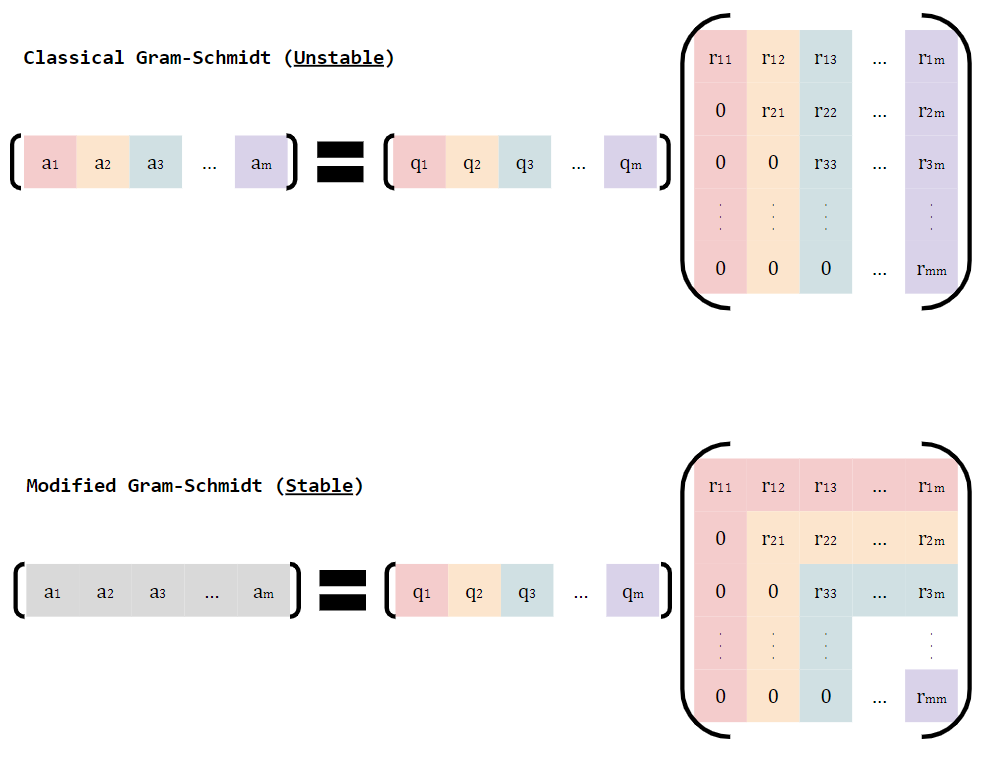
\includegraphics[scale=0.75]{assets/gram.png}
\end{center}

\subsubsection{MATLAB Code}
\begin{mdframed}
    \begin{verbatim}
function [Q,R]=classicalGS(A)         % classical Gram-Schmidt

n = size(A,2);                        % number of columns; this formulation
                                      % does not need the number of rows
for i=1:n                             
Q(:,i) = A(:,i);                      % initialization
   
    for j=1:(i-1)
        R(j,i)=(A(:,i))'*Q(:,j);      % computing R(j,i) by going down the column
        Q(:,i)=Q(:,i)-R(j,i)*Q(:,j);  % updating Q(:,j)
    end
   
    R(i,i) = norm(Q(:,i));            % computing R(i,i) 
    Q(:,i)=Q(:,i)/R(i,i);             % making Q(:,i) a unit vector
end
    \end{verbatim}
\end{mdframed}


\subsection{Modified Gram-Schmidt}
As mentioned earlier, the modified Gram-Schmidt is a stable algorithm that builds $R$ one row at a time. 

\subsubsection{MATLAB Code}
\begin{mdframed}
    \begin{verbatim}
function [Q,R]=modifiedGS(A)          % modified Gram-Schmidt

n = size(A,2);                        % number of columns; this formulation
                                      % does not need the number of rows
for i=1:n                             
    Q(:,i) = A(:,i);                  % initialization
end

for i=1:n
    R(i,i) = norm(Q(:,i));            % computing R(i,i) 
    Q(:,i)=Q(:,i)/R(i,i);             % making Q(:,i) a unit vector

    for j=(i+1):n
        R(i,j)=(Q(:,i))'*Q(:,j);      % computing R(i,j) by going right on ith row
        Q(:,j)=Q(:,j)-R(i,j)*Q(:,i);  % updating Q(:,j)
    end

end
    \end{verbatim}
\end{mdframed}

\subsubsection{Worked Example}
We'll base our algorithm on the MATLAB code above. 
\begin{mdframed}
    (Example.) We'll solve the same problem as in the previous example, \emph{except} we'll use the modified algorithm instead. To reiterate, suppose we have \[A = \begin{bmatrix}
        -1 & -1 & 1 \\ 
        1 & 3 & 3 \\ 
        -1 & -1 & 5 \\ 
        1 & 3 & 7
    \end{bmatrix}.\]
    We can define 
    \[\vec{a_1} = \begin{bmatrix}
        -1 \\ 1 \\ -1 \\ 1
    \end{bmatrix} \quad \vec{a_2} = \begin{bmatrix}
        -1 \\ 3 \\ -1 \\ 3
    \end{bmatrix} \quad \vec{a_3} = \begin{bmatrix}
        1 \\ 3 \\ 5 \\ 7
    \end{bmatrix}.\]
    In other words, our goal is to get something like 
    \[A = \begin{bmatrix}
        a_1 & a_2 & a_3
    \end{bmatrix} = \begin{bmatrix}
        q_1 & q_2 & q_3
    \end{bmatrix} \begin{bmatrix}
        r_{11} & r_{12} & r_{13} \\ 
        0 & r_{22} & r_{23} \\ 
        0 & 0 & r_{33}
    \end{bmatrix}.\]
    \textbf{Keep this in mind}, since we'll be assuming this. Then, we can find the elements of $\hat{Q}$ and $\hat{R}$. We'll run through the algorithm described in code above. 
    \begin{enumerate}
        \item First, we define $q_1 = a_1$, $q_2 = a_2$, and $q_3 = a_3$. 
        
        \item Next, for we want to find $r_{11}$, $r_{12}$, $r_{13}$ and then determine $q_1$. We can also update $q_2$ and $q_3$. 
        
        \begin{itemize}
            \item (Outer Loop: $i = 1$.) Note that 
            \[r_{11} = ||q_1||_2 = ||a_1||_2 = \sqrt{(-1)^2 + 1^2 + (-1)^2 + 1^2} = 2.\]
            Here, $r_{11} = ||q_1||_2$ comes from the algorithm (since we \emph{initially} set $q_1 = a_1$.)
            \[q_1 = \frac{q_1}{r_{11}} = \frac{q_1}{||a_1||_2} = \begin{bmatrix}
                -1/2 \\ 1/2 \\ -1/2 \\ 1/2
            \end{bmatrix}.\]
            Here, we've updated the value of $q_1$. 
    
            \item In the \emph{inner loop}, we do the following for $j = 2$ to $3$:
            \begin{itemize}
                \item (Inner Loop: $j = 2$.) Next, note that 
                \[r_{12} = \cyclic{q_1, q_2} = q_1^T q_2 = q_1^T a_2 = \left(-\frac{1}{2}\right)(-1) + \frac{1}{2}(3) + \left(-\frac{1}{2}\right)(-1) + \frac{1}{2}(3) = 4.\]
                From there, it follows that 
                \[q_2 = q_2 - r_{12}q_1 = \begin{bmatrix}
                    -1 \\ 3 \\ -1 \\ 3
                \end{bmatrix} - 4 \begin{bmatrix}
                    -1/2 \\ 1/2 \\ -1/2 \\ 1/2
                \end{bmatrix} = \begin{bmatrix}
                    1 \\ 1 \\ 1 \\ 1
                \end{bmatrix}.\]
        
                \item (Inner Loop: $j = 3$.) Next, we have 
                \[r_{13} = \cyclic{q_1, q_3} = q_1^T q_3 = q_1^T a_3 = \left(-\frac{1}{2}\right)(1) + \frac{1}{2}(3) + \left(-\frac{1}{2}\right)(5) + \frac{1}{2}7 = 2.\]
                From there, it follows that 
                \[q_3 = q_3 - r_{13}q_1 = \begin{bmatrix}
                    1\\3\\5\\7
                \end{bmatrix} - 2\begin{bmatrix}
                    -1/2 \\ 1/2 \\ -1/2 \\ 1/2
                \end{bmatrix} = \begin{bmatrix}
                    2 \\ 2 \\ 6 \\ 6
                \end{bmatrix}.\]
            \end{itemize}
        \end{itemize}
        
        \item After running through the first iteration of the outer loop discussed in the algorithm, we have 
        \[q_2 = \begin{bmatrix}
            1\\1\\1\\1
        \end{bmatrix} \quad q_3 = \begin{bmatrix}
            2\\2\\6\\6
        \end{bmatrix}.\] 
        Now, we want to find $r_{22}$, $r_{23}$, and determine $q_2$. We also update $q_3$. 
        \begin{itemize}
            \item (Outer Loop: $i = 2$.) We have 
            \[r_{22} = ||q_2||_2 = \sqrt{1^2 + 1^2 + 1^2 + 1^2} = 2.\]
            So, updating $q_2$ gives us 
            \[q_2 = \frac{q_2}{r_{22}} = \begin{bmatrix}
                1/2 \\ 1/2 \\ 1/2 \\ 1/2
            \end{bmatrix}.\] 

            \item In the \emph{inner loop}, we do the following for $j = 3$ to $3$:
            \begin{itemize}
                \item (Inner Loop: $j = 3$.) We have 
                \[r_{23} = \cyclic{q_2, q_3} = q_2^T = q_3 = \frac{1}{2}(2) + \frac{1}{2}(2) + \frac{1}{2}(6) + \frac{1}{2}(6) = 8.\]
                From there, 
                \[q_3 = q_3 - r_{23}q_2 = \begin{bmatrix}
                    2\\2\\6\\6
                \end{bmatrix} - 8\begin{bmatrix}
                    1/2 \\ 1/2 \\ 1/2 \\ 1/2
                \end{bmatrix} = \begin{bmatrix}
                    -2 \\ -2 \\ 2 \\ 2
                \end{bmatrix}.\]
            \end{itemize}
        \end{itemize}

        \item After running through the second iteration of the outer loop discussed in the algorithm, we have 
        \[q_3 = \begin{bmatrix}
            -2 \\ -2 \\ 2 \\ 2
        \end{bmatrix}.\]
        Now, we can find $r_{33}$ and determine the value of $q_3$. 
        \begin{itemize}
            \item (Outer Loop: $i = 3$.) We have 
            \[r_{33} = ||q_3||_2 = \sqrt{(-2)^2 + (-2)^2 + 2^2 + 2^2} = 4.\]
            So, 
            \[q_3 = \frac{q_3}{r_{33}} = \begin{bmatrix}
                -1/2 \\ -1/2 \\ 1/2 \\ 1/2
            \end{bmatrix}.\]

            \item Notice that the inner loop is not executed since $j = 4$ is greater than $3$.
        \end{itemize}
    \end{enumerate}
\end{mdframed}





\end{document}